%% inicio, la clase del documento es iccmemoria.cls
\documentclass{iccmemoria}
\usepackage[onelanguage, commentsnumbered, linesnumbered, boxed, ruled]{algorithm2e}
\usepackage{pdfpages}
\usepackage{amsfonts}
\usepackage{amssymb}
\usepackage{amsmath}
\usepackage{array}
\usepackage{longtable}
\usepackage{float}
\usepackage{especificacionutility}
\usepackage{enumitem}
\usepackage{listings}

\lstset{ %
    language=Java, % lenguaje
    basicstyle=\bfseries\ttfamily,
    % keywordstyle=\color{blue},
    % commentstyle=\color{brown},
    % backgroundcolor=\color{gray!10},
    showstringspaces=false,
    frame=tb,
    xleftmargin=3.4pt,
    xrightmargin=3.4pt,
    breaklines=true,
}

%% datos generales y para la tapa
\titulo{Herramienta para la optimizaci�n de redes de distribuci�n de agua potable}
\author{Gabriel Gonzalo Alexander Sanhueza Fuentes}
\supervisor{Jimmy Guti�rrez Bahamondes}
\cosupervisor{Daniel Mora Melia}
\informantes
	{Profesor Informante 1}
	{Profesor Informante 2}
\adicional{(s�lo por si se necesita agregar alg�n otro profesor)}
\director{Profesor del ramo Memoria de T�tulo}
\date{08, 2020}

%% inicio de documento
\begin{document}

%% crea la tapa
\maketitle

%% dedicatoria
\begin{dedicatory}
Dedicado a ...
\end{dedicatory}

%% agradecimientos
\begin{acknowledgment}
Agradecimientos a ...
\end{acknowledgment}

%% indices
\tableofcontents
\listoffigures
\listoftables

%% resumen
\input{Resumen/Resumen}

%% abstract

\chapter{Introducci�n}
El proyecto que se desarrollara consiste en la creaci�n de una herramienta que haga uso de algoritmos metaheur�sticos para tratar y minimizar problemas existentes en redes de distribuci�n de agua potable.

Este proyecto solo abarcara dos problemas existentes dentro de las redes de distribuci�n de agua potable.

Para el desarrollo de este proyecto se usar�n librer�as ya existentes con el fin de reducir el tiempo de desarrollo. Estas librer�as son epanet2.dll, desarrollada en c, y JNA, librer�a en java para funciones nativas.


\section{Prop�sito del Sistema}

El proyecto consiste en el desarrollo de un sistema que permite simular y buscar soluciones a problemas presentes en las redes de distribuci�n de agua potable haciendo uso de algoritmos metaheur�sticos. Adicionalmente, el sistema es dise�ado de tal forma que pueda ser extendido a�adiendo nuevos problemas, algoritmos u operadores.
\section{Alcance del proyecto}

Al final del periodo de desarrollo la herramienta contara con las siguientes prestaciones.

\begin{itemize}
    \item	El sistema permitir� la carga y la visualizaci�n de la red gr�ficamente.
    \item	El sistema solo resolver� dos clases de problemas de optimizaci�n, uno mono-objetivo y el otro multiobjetivo. El problema mono-objetivo ser� el de los costos de inversi�n. En cuanto al problema multiobjetivo, este ser� el de los costos energ�ticos y el n�mero de encendidos y apagado de las bombas.  
    \item	El sistema �nicamente contara con dos algoritmos implementados los cuales ser�n el algoritmo gen�tico y NSGA-II. El algoritmo gen�tico ser� el usado para tratar el problema mono-objetivo, mientras que NSGA-II ser� aplicado al multiobjetivo.
    \item	El sistema permitir� visualizar y guardar las soluciones de los algoritmos en un archivo.
    \item	El sistema permitir� que el usuario agregue nuevos algoritmos, operadores o problemas sin tener que modificar la interfaz de usuario.
\end{itemize}

Este proyecto no contempla la creaci�n de la red por lo que estas deber�n ser ingresadas como entradas al programa. 

Adem�s, esta herramienta �nicamente podr� ser ocupada en equipos cuyo sistema operativo sea Windows debido a que se realizan llamadas a librer�as nativas.

\section{Contexto}

Este sistema ser� desarrollado utilizando el lenguaje de programaci�n java. Debido a que este es un lenguaje ampliamente utilizado y que cuenta con un gran soporte y comunidad que lo utilizan.

Como motor de c�lculo para llevar a cabo las simulaciones se utilizar� una librer�a desarrollada en c, que cuenta con funciones para llevar a cabo simulaciones de redes de agua potable. El nombre de esta librer�a es epanet2.dll. Las funciones que incorpora esta librer�a se encuentran explicadas en~\cite{Rossman2017}.

Desde lenguaje se realizar�n llamadas a librer�as nativas usando la librer�a JNA existente en java. Esta librer�a cuenta con las clases y m�todos necesarios para poder acoplar este sistema a la librer�a epanet2.dll desarrollada en c y que ser� usada como motor de c�lculo para llevar a cabo las simulaciones.
Puesto que una de las funcionalidades del sistema es permitir la ejecuci�n de algoritmos metaheur�sticos, se toma como base la arquitectura presentada por el framework JMetal.

JMetal es un framework para la optimizaci�n multiobjetivo con metaheur�sticas. Su arquitectura inicial~\cite{Durillo2010} involucraba una serie de problemas y dificultaban la realizaci�n de ciertas acciones que eran recurrentes. Adem�s, esta no hacia uso de las novedades incorporadas por Java como los gen�ricos. Es por esto, que posteriormente fue redise�ada, haciendo uso de patrones de dise�o, principios de la programaci�n orientada a objetos y aprovechando las caracter�sticas del lenguaje Java. Este redise�o se presenta en~\cite{Nebro2015}.

El contexto en el que se desenvolver� este sistema ser� en ambientes universitario, de investigaci�n y en el ambiente laboral. 

\section{Definiciones, Acr�nimos y Abreviaturas}

NSGA-II: Non-dominated Sorting Genetic Algorithm
%% genera las referencias
\bibliography{refs}
\chapter{Marco Te�rico}
En este cap�tulo se presentan los conceptos que ser�n necesarios para la realizaci�n del proyecto.

\section{Metodolog�a de desarrollo}
Para el desarrollo de este proyecto se opto por la metodolog�a iterativa e incremental.

\subsection{Metodolog�a iterativa e incremental}
La metodolog�a iterativa e incremental lleva a cabo el desarrollo de un proyecto de software dividi�ndolo en iteraciones que generan un incremento, el cual contribuye en el desarrollo del producto final.

Cada iteraci�n se compone de las fases de an�lisis, dise�o, implementaci�n y pruebas como se muestra en la Figura \ref{fig:methodie}. La fase de an�lisis se encarga de llevar a cabo la obtenci�n y definici�n de los requerimientos del software. Durante la etapa de dise�o se realiza la conceptualizaci�n del software basado en los requerimientos definidos anteriormente. Durante la implementaci�n se codifican las funcionalidades siguiendo las directivas establecidas durante el dise�o, con el fin de satisfacer los requerimientos. Y finalmente, durante la fase de pruebas, se valida y verifica la correctitud de las funcionalidades implementadas, as� como el cumplimiento de los requisitos.

\begin{figure}[h]
	\includegraphics{Capitulo2/assets/iedevelopment.eps}
	\centering
	\caption{Metodolog�a iterativa e incremental \cite{Pressman2009}}
	\label{fig:methodie}
\end{figure}

El hecho de llevar a cabo un desarrollo iterativo permite la obtenci�n de retroalimentaci�n del producto que se esta desarrollando tempranamente y de esta manera poder refinar el trabajo en etapas posteriores del desarrollo. \cite{Victor2003, Mitchell2009, Martin1999,Alshamrani2015}.

\section{Metodolog�a de evaluaci�n}
\subsection{Estudio de caso}
Un estudio de caso~\cite{Runeson2009} es una metodolog�a de investigaci�n la cual en ingenier�a de software permite analizar un proyecto, un grupo de personas, un producto, etc, en un contexto real con el objetivo de responder la pregunta de investigaci�n planteada. Esta metodolog�a de evaluaci�n considera aspectos formales para obtener evidencia. Las actividades para llevar a cabo el estudio de caso se pueden dividir en las siguientes categor�as:


\begin{itemize}
	\item Dise�o del estudio de caso: 
	\begin{itemize}
		\item Elecci�n del caso: Consiste en definir el objeto a estudiar. Este puede ser un proceso, producto, grupo de persona, etc.
		%\item Describir el contexto de aplicaci�n del caso: Consiste en establecer sobre que elemento se aplicar� el estudio de caso a desarrollar.
		\item Definici�n de objetivos experimentales: Consiste en indicar cual es el objetivo de la investigaci�n a realizar, si es describir, evaluar o explicar alg�n suceso.
		\item Definici�n de un protocolo para conducir el estudio de caso: Consiste en escoger las pautas para llevar a cabo el estudio de caso, que instrumentos ser�n utilizados para recolectar datos y como se realizaran el an�lisis de estos.
		\item Definici�n de caracter�sticas a evaluar: Consiste en establecer qu� es lo que estamos interesados en evaluar del elemento sobre el que se aplica el estudio de caso.
		\item Definici�n de sujetos de prueba: Consiste en indicar cual sera la fuente de datos a ser utilizada para el estudio de caso, estas pueden ser personas, datos ya recolectados, etc.
	\end{itemize}
	\item Recolecci�n de datos:
	\begin{itemize}
		\item Aplicaci�n de estudio de caso en un conjunto de sesiones no controladas: Consiste en llevar a cabo el estudio de caso sobre los sujeto de prueba definidos.
	\end{itemize}
	\item An�lisis de los datos recolectados:
	\begin{itemize}
		\item Aplicaci�n de herramientas de obtenci�n de evidencia emp�rica: Consiste en la utilizaci�n de m�todos o t�cnicas con el fin de obtener evidencia emp�rica a partir de los datos recolectados.
		\item An�lisis y evaluaci�n de datos emp�ricos: Consiste en analizar la evidencia y evaluar la validez de los resultados obtenidos.
	\end{itemize}
	\item Reportar los resultados del estudio de caso:
	\begin{itemize}
		\item Presentar los resultados y las conclusiones del estudio de caso.
	\end{itemize}
	
	
\end{itemize}
% \begin{itemize}
% 	\item Describir el contexto de aplicaci�n del caso: Consiste en establecer sobre que elemento se aplicar� el estudio de caso a desarrollar.
% 	\item Definici�n de objetivos experimentales: Consiste en indicar cual es el objetivo de la investigaci�n a realizar, si es describir, evaluar o explicar alg�n suceso.
% 	\item Definici�n de un protocolo para conducir el estudio de caso: Consiste en escoger las pautas para llevar a cabo el estudio de caso, que instrumentos ser�n utilizados para recolectar datos y como se realizaran el an�lisis de estos.
% 	\item Definici�n de caracter�sticas a evaluar: Consiste en establecer qu� es lo que estamos interesados en evaluar del elemento sobre el que se aplica el estudio de caso.
% 	\item Definici�n de sujetos de prueba: Consiste en indicar cual sera la fuente de datos a ser utilizada para el estudio de caso, estas pueden ser personas, datos ya recolectados, etc.
% 	\item Aplicaci�n de estudio de caso en un conjunto de sesiones no controladas: Consiste en llevar a cabo el estudio de caso sobre los sujeto de prueba definidos.
% 	\item Aplicaci�n de herramientas de obtenci�n de evidencia emp�rica: Consiste en la utilizaci�n de m�todos o t�cnicas con el fin de obtener evidencia emp�rica a partir de los datos recolectados.
% 	\item An�lisis y evaluaci�n de datos emp�ricos: Consiste en analizar la evidencia y evaluar la validez de los resultados obtenidos.
% \end{itemize}

\section{Herramientas para el desarrollo del software}
A continuaci�n se presentan las herramientas utilizadas para el desarrollo del proyecto.

\subsection{Lenguaje de programaci�n Java}
Java es un lenguaje de programaci�n de alto nivel orientado a objetos y de prop�sito general. Fue anunciado por Sun Microsystems en Mayo de 1995~\cite{3Java}. Un programa Java se ejecuta sobre la maquina virtual llamada la \textit{Java Virtual Machine}, la cual le da a este lenguaje la caracter�stica de ser multiplataforma. Adicionalmente, Java incorpora el soporte para multi-hilos, una poderosa herramienta que permite la ejecuci�n de distintas instrucciones de c�digo al mismo tiempo~\cite{Gosling2015}. Ademas. este lenguaje tambi�n posee una caracter�stica conocida como el recolector de basura, que se encarga de limpiar la memoria de objetos que ya no est�n siendo utilizados. 

La elecci�n de Java como lenguaje de programaci�n para desarrollar este proyecto fue un requerimiento de los investigadores que participan del proyecto ya que permite la incorporaci�n directa de algunas herramientas que han sido dise�adas.

A continuaci�n se describen las funcionalidades de Java que han sido m�s importantes para desarrollar este trabajo.

\subsubsection{Java Reflection}
Caracter�stica de Java que permite que un programa se auto examine. Esta caracter�stica est� disponible a trav�s de la \textit{Java Reflection API}, la cual cuenta con m�todos para obtener los metadatos de las clases, m�todos, constructores, campos o par�metros. Esta API tambi�n permite crear nuevos objetos cuyo tipo era desconocido al momento de compilar el programa~\cite{Braux1999}.

\subsubsection{Java Annotation}
Caracter�stica de Java para agregar metadatos a elementos del lenguaje como las clases, m�todos, par�metros, etc~\cite{Rocha2011}. Las anotaciones no tienen efecto directo sobre el c�digo. Sin embargo, combinadas con \textit{Java Reflection} permiten realizar una serie de tareas muy �tiles como crear nuevos objetos cuyo tipo no conocemos en tiempo de compilaci�n.

Las anotaciones est�n presentes en varios lenguajes como Python y C\#, siendo en este �ltimo llamadas Atributos. Generalmente, los lenguajes que incorporan anotaciones tambi�n implementan la t�cnica llamada reflexi�n.

A continuaci�n se presenta un ejemplo de la anotaci�n \textit{@Override} en Java:

\begin{lstlisting}
    @Override
    public void toString(){}
\end{lstlisting}

\subsubsection{Polimorfismo}
El polimorfismo es la t�cnica que permite modificar el comportamiento de un elemento del lenguaje~\cite{Cardelli-1985}, sea este una clase, funci�n, m�todo u operador, dependiendo del tipo de dato real con el que se esta trabajando. Existen muchas formas de polimorfismo. Las principales son nombrados a continuaci�n usando su nombre en �ngles:

\begin{itemize}
    \item \textit{Universal Polymorphism}: Son aquellas t�cnicas que trabajar sobre un cualquier tipo de instancia con una estructura com�n, es por ello que pueden emplear la misma operaci�n sin cambios en el c�digo.
    \begin{itemize}
        \item \textit{Parametric polymorphism}: Se refiere al uso de una funci�n u objeto sin importar el tipo de instancia sobre la que trabaja, es decir, opera de manera uniforme los distintos tipos que desea operar. Las funciones que cuentan con este tipo de polimorfismo se conoce tambi�n como funciones gen�ricas. A modo de ejemplo se encuentran los gen�ricos de Java y los \textit{templates} de C++.
        \item \textit{Inclusion}: Hace referencia a los subtipos. En donde una clase puede ser usado y manipulado donde quiera que se espere el supertipo de �sta.
    \end{itemize}
    \item \textit{Ad-hoc polymorphism}: Estas t�cnicas trabajan sobre un conjunto limitado de tipos que no est�n relacionados, necesitando manejar cada tipo de manera diferente.
    \begin{itemize}
        \item \textit{Overloading}: Hace referencia a la reutilizaci�n de s�mbolos o nombres de funciones en m�s de un contexto. Por ejemplo, algunos lenguajes permiten usar el mismo nombre de funci�n variando el n�mero de argumentos recibidos o el tipo de ellos. Tambi�n se cuenta la sobrecarga de los operadores que permiten algunos lenguajes como C++.
        \item \textit{Coercion}: Este tipo de polimorfismo hace referencia a la conversi�n autom�tica de tipos. Por ejemplo, al sumar un valor entero y un real en algunos lenguaje de programaci�n, el valor entero es convertido a real antes de aplicar el operador de la suma.
    \end{itemize}
\end{itemize}
Java incorpora variaciones de los tipos anteriormente mencionados de polimorfismo.

\subsection{Patrones de dise�o}
En esta secci�n se describen los patrones de dise�o que fueron m�s importantes durante la realizaci�n del proyecto.

\subsubsection{Inversi�n de control}
La Inversi�n de Control~\cite{State2020} es un principio de ingenier�a de software en que el control se transfiere desde el programador al programa, permitiendo as� sistemas con menor acoplamiento. Utilizando este principio se establece un flujo de ejecuci�n en la aplicaci�n en el cual se incorporan las llamadas al c�digo implementado por el cliente. Esta t�cnica es ampliamente usada en los \textit{frameworks}. Dos ejemplos de framework que usan esta t�cnica son Spring en Java y Angular en JavaScript \cite{Hudli2013}.

\subsubsection{Inyecci�n de dependencias}
La Inyecci�n de Dependencias (DI)~\cite{State2020}, es un patr�n de dise�o que permite reducir el acoplamiento entre los componentes dejando la tarea de crear las dependencias de un objeto en manos de un externo, el cual podr�a ser un modulo dentro del programa, para posteriormente enviarla a la instancia que la requiera. Este es una de las t�cnicas utilizadas para implementar el principio de inversi�n de control en un sistema. De acuerdo a \cite{Hudli2013} la inyecci�n de dependencias presenta los siguientes problemas~\cite{Hudli2013}:

\begin{itemize}
    \item Las dependencias inyectadas deben ser compatibles con la abstracci�n definida en la clase, es decir, la instancia a inyectar debe ser un subtipo de la clase esperada.
    \item Las clases que se inyectan deben implementar el comportamiento que espera la clase que hace uso de esta dependencia.
\end{itemize}

\subsection{Epanet Programming Toolkit}
% Software que permite simular el comportamiento hidr�ulico y la calidad del agua en redes de distribuci�n de aguas compuesta por tuber�as, nodos, bombas, v�lvulas y tanques de almacenamiento~\cite{Rossman2017}.  Este software cuenta tambi�n con una librer�a din�mica conocida bajo el nombre de Epanet Programming Toolkit, la cual cuenta con un conjunto de funciones para realizar simulaciones desde diferentes entornos de desarrollo como C, C++, VB, Java, etc~\cite{Rossman1999}.

Librer�a de enlace din�mico que permite realizar simulaciones computaciones del comportamiento del agua en RDA. Esta librer�a es parte de Epanet, un software que permite simular el comportamiento hidr�ulico y la calidad del agua en redes de distribuci�n de aguas compuesta por tuber�as, nodos, bombas, v�lvulas y tanques de almacenamiento~\cite{Rossman2017}. Fue creada por la agencia EPA de EE.UU. La librer�a cuenta con un conjunto de funciones para realizar simulaciones desde diferentes entornos de desarrollo como C, C++, VB, Java, etc~\cite{Rossman1999}.
\section{Red de distribuci�n de agua potable}
Conjunto de elementos enlazados de tal manera que permite suministrar cierta cantidad de agua a una presi�n establecida~\cite{Doctoral2012}.

\subsubsection{Caudal}
Cantidad de agua que se mueve a trav�s de un segmento de la red.

\subsection{Componentes f�sicos de una red}
A continuaci�n se define los componentes que conforman una red de agua potable~\cite{Rossman2017}, los cuales se aprecian en la Figura~\ref{fig:componentesfisicos}:


\begin{figure}[h]
	 \includegraphics{Capitulo2/assets/componentesfisicosred.eps}
	\centering
	\caption{Componentes f�sicos de un sistema de distribuci�n de agua~\cite{Rossman2017}}
	\label{fig:componentesfisicos}
\end{figure}
\subsubsection{Nudos de caudal}

Son los puntos o extremos de una tuber�a, los cuales tambi�n permiten que estas se unan. Estos nudos pueden actuar como nudos de demanda a trav�s de los cuales el flujo abandona la red.

\subsubsection{Embalse}
Es una fuente de alimentaci�n externa.
\subsubsection{Deposito}
Son elementos con la capacidad de almacenar agua.
\subsubsection{Tuber�a}
 Son los elementos a trav�s de los cuales transita el agua de un nudo a otro.
\subsubsection{Bomba}
Elementos que permiten impulsar el liquido con el fin de elevarlo a una posici�n superior.
\subsubsection{V�lvula}
Elementos que limitan la presi�n o el caudal que transita en un punto de la red.
\subsection{Epanet}
Software que permite simular el comportamiento hidr�ulico y la calidad del agua en redes de distribuci�n de aguas compuesta por tuber�as, nodos, bombas, v�lvulas y tanques de almacenamiento~\cite{Rossman2017}.  Este software cuenta tambi�n con una librer�a din�mica conocida bajo el nombre de Epanet Programming Toolkit, la cual cuenta con un conjunto de funciones para realizar simulaciones desde diferentes entornos de desarrollo como C, C++, VB, Java, etc~\cite{Rossman1999}.
\section{Optimizaci�n}
La optimizaci�n consiste en maximizar o minimizar un conjunto de funciones que matem�ticamente pueden ser expresadas de la siguiente forma:
$$f_1(x),f_2(x), ..., f_N(x),\ x=(x_1,...,x_d) | x \in X$$
sujeto a una serie de condiciones
$$h_j(x) = 0, j=1,2,...,J$$
$$g_k(x) \leq 0, k=1,2,...,K$$
siendo $f_1,...,f_N$ funciones objetivos; $x_1, ..., x_d$ variables de decisi�n, pertenecientes al espacio de b�squeda $X$; y $h_j$ junto con $g_k$, una serie de restricciones~\cite{Yang2015}. De acuerdo a la cantidad de funciones objetivos que se tenga, se establece que si $N=1$ la optimizaci�n es \textbf{monoobjetivo}, mientras que para $N\geq 2$ se conoce como \textbf{multiobjetivo}~\cite{Yang2015}. En este punto se debe tener en cuenta que los objetivos planteados deben encontrarse en contradicci�n. 

Debido a la definici�n de las restricciones es posible dividir el espacio de b�squeda en dos regiones~\cite{Bozorg-Haddad2017}:
\begin{itemize}
	\item Soluciones factibles: Compuesto por los elementos pertenecientes al espacio de b�squeda que satisfacen todas las restricciones.
	\item Soluciones no factibles: Integrado por aquellos elementos que no cumplen todas las restricciones.
\end{itemize}
\section{Heur�stica}
Es el conocimiento que se tiene del problema el cual permite acotar la b�squeda de las soluciones en espacios de b�squeda de gran tama�o que hacen inviable la aplicaci�n de t�cnicas deterministas por el costo de tiempo que implican. Con la utilizaci�n de estas t�cnicas se espera encontrar soluciones buenas en un tiempo razonable, pero esto no esta garantizado \cite{Yang2015,Romanycia1985}.
\section{Metaheur�stica}
Algoritmos que permiten resolver un amplio rango de problemas de optimizaci�n empleando t�cnicas con alg�n grado de aleatoriedad para encontrar soluciones a un problema. Estos algoritmos no garantizan que la soluci�n encontrada sea la �ptima, pero permiten obtener generalmente aproximaciones a �sta. La diferencia entre heur�sticas y metaheur�sticas, es que esta �ltima puede ser aplicado a un amplio conjunto de problemas sin necesidad de realizar grandes cambios en el algoritmo, mientras que las heur�sticas generalmente son aplicadas a un dominio especifico~\cite{Yang2015,Boussaid2013,Luke2013}.

\section{Algoritmos Evolutivos}
Conjunto de algoritmos inspirado en la teor�a de la evoluci�n de Darwin acerca de la capacidad de la naturaleza para evolucionar seres vivos bien adaptados a su entorno. Estos algoritmos hacen uso de diversos mecanismos entre los que se encuentra la selecci�n, mutaci�n y cruzamiento sobre los individuos de una poblaci�n con el fin de generar una nueva generaci�n de individuos~\cite{Boussaid2013}.

\subsection{Conceptos Generales}

\subsubsection{Individuo} 
Representa una soluci�n al problema. Los individuos pueden ser representados de diversas manera. El proceso mediante se realiza este mapeo, se denomina c�dificaci�n. Se ha demostrado que la selecci�n de una codificaci�n u otra influye directamente en los resultados dependiendo del problema estudiado, entre �stas se encuentra la representaci�n binaria (1 y 0), la real (utilizando n�meros reales), etc. Para la representaci�n binaria cada variable se codifica como un conjunto de bits, lo cual forma una cadena binaria. Por ejemplo, la representaci�n binaria de la soluci�n $(2,4,6,8)$ formada por enteros de 4 bits corresponder�a a

$$0010\ 0100\ 0110\ 1000$$


En cambio, para la representaci�n real esta se presenta como un vector, en donde cada valor que forma este vector pertenece a los n�meros reales, es decir, 
$$v = (x1,x2, \dots, x_n), \textrm{en donde } v \in \mathbb{R}^n$$

\subsubsection{Poblaci�n} 
Conjunto de  individuos (soluciones) candidatos sobre las cual opera el algoritmo. Durante cada iteraci�n del algoritmo se generan nuevas soluciones que son agregadas a la poblaci�n a la vez que se remueven otras seg�n cada estrateg�a~\cite{Heiss-Czedik1997}.

\subsubsection{Etapas de un algoritmo evolutivo}
\begin{itemize}
	\item \textbf{Selecci�n:} La selecci�n es un mecanismo utilizado por los algoritmos evolutivos para escoger a los individuos mas aptos los cuales ser�n usados para la reproducci�n~\cite{Heiss-Czedik1997}. Existen numerosos algoritmos de selecci�n que pueden ser utilizados en los algoritmos evolutivos.
	\item \textbf{Reproducci�n:} La reproducci�n es el proceso en el cual de combinan individuos con el fin de mantener la diversidad de las soluciones y generar las nuevas generaciones.
\end{itemize}

\subsubsection{Operadores} 
Estos procedimientos permiten generar diversidad en las soluciones y a la vez explotar las mejores caracter�sticas de los individuos.

\subsubsection{Operadores generales:}
\begin{itemize}
	\item \textbf{Cruzamiento:} El cruzamiento es un mecanismo usado para generar nuevos soluciones a partir de dos o mas individuos seleccionados~\cite{Blum2003, Boussaid2013}. En la Figura~\ref{fig:crossover} se aprecia un cruce entre dos individuos en torno a un punto de cruzamiento.
	\begin{figure}[H]
		\centering
		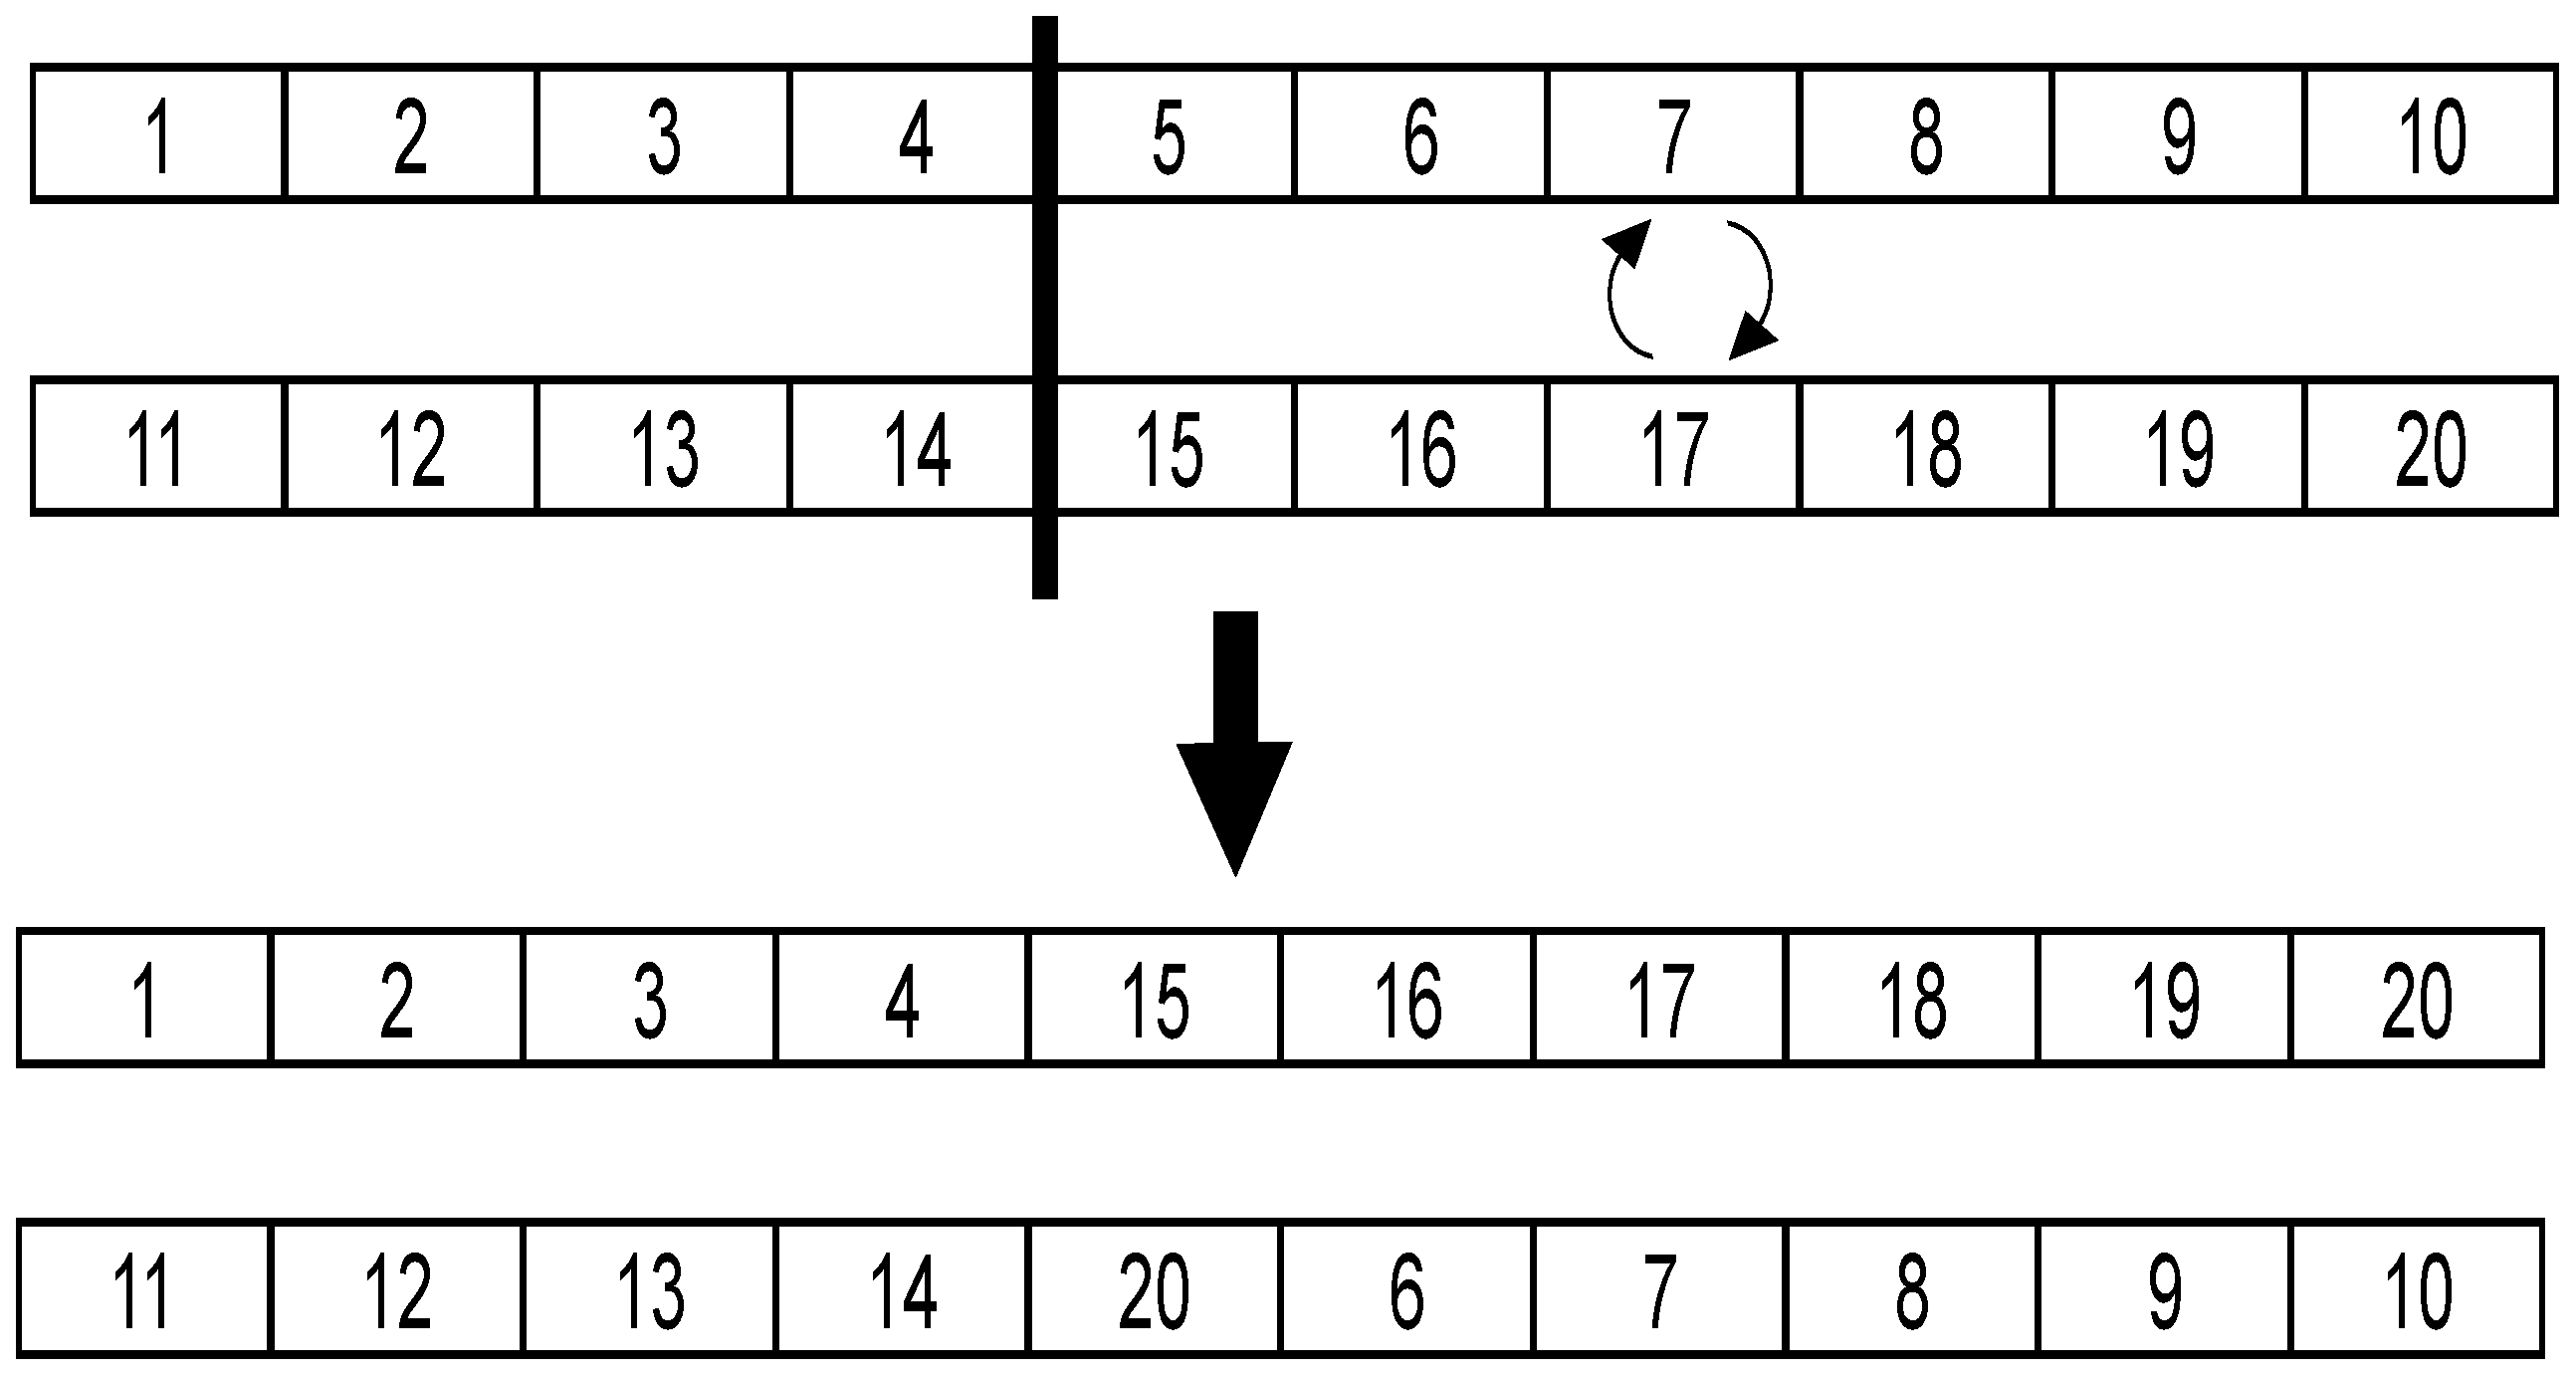
\includegraphics[width=0.5\textwidth]{Capitulo2/assets/Crossover.eps}
		\caption{Cruzamiento en un punto}
		\label{fig:crossover}
	\end{figure}
	\item \textbf{Mutaci�n:} La mutaci�n es un operador el cual permite mantener la diversidad en la descendencia~\cite{Boussaid2013} realizando modificaciones en ciertas partes de la soluci�n. En la FIgura~\ref{fig:mutation} se puede ver una mutaci�n aleatoria en un individuo codificados con n�meros enteros.
	\begin{figure}[H]
		\centering
		\includegraphics[width=0.6\textwidth]{Capitulo2/assets/Mutation.eps}
		\caption{Mutaci�n aleatoria}
		\label{fig:mutation}
	\end{figure}
\end{itemize}

En la Figura~\ref{fig:EA} muestra el pseudoc�digo de los pasos generales de un algoritmo evolutivo.


%\begin{figure}[h]
%	\begin{algorithm}[H]
%		\caption{Algoritmo Evolutivo}
%		\DontPrintSemicolon
%		\SetKwFunction{CreateInitialPopulation}{createInitialPopulation}
%		\SetKwFunction{EvaluatePopulation}{evaluatePopulation}
%		\SetKwFunction{Selection}{selection}
%		\SetKwFunction{Crossover}{crossover}
%		\SetKwFunction{Mutation}{mutation}
%		\SetKwFunction{Replace}{replace}
%		\SetKwData{PopulationVar}{population}
%		\SetKwData{SelectionVar}{selection}
%		\SetKwData{OffspringVar}{offspringPopulation}
%		
%		\PopulationVar $\leftarrow$ \CreateInitialPopulation{}\;
%		\EvaluatePopulation{\PopulationVar}\;
%		
%		\While{is not stopping condition reached}{
%			\SelectionVar $\leftarrow$ \Selection{\PopulationVar}\;
%			\OffspringVar $\leftarrow$ \Crossover{\SelectionVar}\;
%			\OffspringVar $\leftarrow$ \Mutation(\OffspringVar)\;
%			\OffspringVar $\leftarrow$ \EvaluatePopulation(\OffspringVar)\;
%			\PopulationVar $\leftarrow$ \Replace(\PopulationVar, \OffspringVar)\;
%		}
%		
%	\end{algorithm}
%	\caption{pseudoc�digo algoritmo evolutivo}
%	\label{fig:EA}
%\end{figure}

\begin{figure}[h]
	\begin{algorithm}[H]
		\caption{Algoritmo Evolutivo}
		\DontPrintSemicolon
		\SetKwFunction{CreateInitialPopulation}{crearPoblaci�nInicial}
		\SetKwFunction{EvaluatePopulation}{evaluarPoblaci�n}
		\SetKwFunction{Selection}{selecci�n}
		\SetKwFunction{Crossover}{cruzamiento}
		\SetKwFunction{Mutation}{mutaci�n}
		\SetKwFunction{Replace}{remplazar}
		\SetKwData{PopulationVar}{poblaci�n}
		\SetKwData{SelectionVar}{poblacionSeleccionada}
		\SetKwData{OffspringVar}{poblaci�nDecendiente}
		
		\PopulationVar $\leftarrow$ \CreateInitialPopulation{}\;
		\EvaluatePopulation{\PopulationVar}\;
		
		\While{la condici�n de termino no ha sido alcanzada}{
			\SelectionVar $\leftarrow$ \Selection{\PopulationVar}\;
			\OffspringVar $\leftarrow$ \Crossover{\SelectionVar}\;
			\OffspringVar $\leftarrow$ \Mutation(\OffspringVar)\;
			\OffspringVar $\leftarrow$ \EvaluatePopulation(\OffspringVar)\;
			\PopulationVar $\leftarrow$ \Replace(\PopulationVar, \OffspringVar)\;
		}
		
	\end{algorithm}
	\caption{Pseudoc�digo Algoritmo Evolutivo}
	\label{fig:EA}
\end{figure}

Primero, se crea la poblaci�n inicial. Despu�s se eval�an los objetivos de dicha poblaci�n y se itera hasta que la condici�n de termino haya sido alcanzada. La condici�n de t�rmino puede ser, por ejemplo un m�ximo numero de evaluaciones o evaluaciones sin mejoras en los resultados.  Dentro del ciclo se realiza la selecci�n sobre la poblaci�n con el fin de determinar las soluciones que ser�n usadas en los operadores de cruzamiento y mutaci�n. Finalmente, se remplaza la poblaci�n inicial con la descendiente.

Dentro de los algoritmos evolutivos m�s utilizados se encuentran el Algoritmo Gen�tico (GA), Programaci�n Gen�tica (GP), Evoluci�n Diferencial (DE), Estrategia Evolutiva (ES) y Programaci�n Evolutiva (EP)~\cite{Slowik-2020}.

Espec�ficamente el GA ha presentado buenos resultados en el �rea de optimizaci�n de RDA~\cite{Doctoral2012}. Es por ello que ha sido seleccionado como uno de los algoritmos para ser implementados en este programa.

\subsection{Algoritmo Gen�tico}
El Algoritmo Gen�tico es uno de los algoritmos evolutivos m�s conocidos y que ha demostrado ser exitoso en una variedad de problemas diferentes. Estos algoritmo hacen uso de los mecanismos de selecci�n y reproducci�n para generar nuevas soluciones a partir de la combinaci�n de otras.

Los individuos en el contexto del Algoritmo Gen�tico son llamados cromosomas, los cuales como se mencion� en la secci�n de los algoritmos evolutivos pueden ser representados de diversas maneras.

% El Algoritmo Gen�tico es una estrategia de b�squeda de soluciones. Para realizar esto, el algoritmo parte desde un conjunto de soluciones denominada poblaci�n he iterativamente, lleva a cabo un proceso de reproducci�n, generando nuevas soluciones~\cite{Heiss-Czedik1997}. Este algoritmo pertenece a la categor�a de algoritmos evolutivos y por lo tanto puede usar el mismo esquema presentado en la Figura~\ref{fig:EA}.



\subsection{Algoritmo NSGAII (\textit{Non-Dominated Sorting Genetic Algorithm II})}
El algoritmo NSGAII~\cite{Deb2002} pertenece a la categor�a de algoritmo evolutivo multiobjetivo (MOEA). Este algoritmo al igual que el Algoritmo Gen�tico hace uso de los operadores de selecci�n, cruzamiento y mutaci�n para encontrar un conjunto de soluciones optimas a problemas que cuentan con m�s de un objetivo. Adicionalmente, NSGAII a�ade conceptos y operadores adicionales los cuales permiten mejorar su rendimiento y la calidad de las soluciones obtenidas. NSGAII puede ser implementado siguiendo los mismos pasos de el algoritmo evolutivo mostrados en la Figura~\ref{fig:EA}, utilizando la funci�n de remplazo mostrada en la Figura~\ref{fig:RemplaceNSGAII}.

En la Figura~\ref{fig:RemplaceNSGAII} se puede ver que el proceso de remplazo dentro del Algoritmo Gen�tico consiste en unir la poblaci�n actual y la poblaci�n descendiente (formada por los elementos resultantes del operador de selecci�n y sobre la que se han aplicado el cruzamiento y la mutaci�n) en un solo elemento llamada unionPoblaci�n. Luego, esta  es enviada a un procedimiento el cual ordena y categoriza la poblaci�n en diversos frentes de acuerdo al concepto de dominancia de Pareto. Despu�s, de que la poblaci�n a sido categorizada se procede a iterar sobre los frentes y a�adir sus elementos a una nueva poblaci�n con el cuidado de no sobrepasar el tama�o de la poblaci�n deseada ($N$). En caso de que uno de los frentes no pueda ser a�adido en su totalidad por sobrepasar dicho tama�o, se llevar� a cabo un proceso por el cual se ordenaran las soluciones en dicho frente basadas en un criterio conocido como densidad de las soluciones. Una vez realizado el ordenamiento, se agregar�n las mejores soluciones a la nueva poblaci�n hasta alcanzar el tama�o deseado  $N$. Se puede ver un ejemplo de este procedimiento gr�ficamente en la Figura~\ref{fig:procedimientoNSGAII}.

% Una vez las soluciones se encuentren ordenadas se rellenar� la nueva poblaci�n hasta alcanzar el tama�o de deseado $N$. 

\begin{figure}[h]
	\begin{algorithm}[H]
		\caption{Funci�n de remplazo para el algoritmo NSGAII}
		\DontPrintSemicolon
		\SetKwData{PopulationVar}{poblaci�n}
		\SetKwData{OffspringVar}{poblaci�nDescendiente}
		\SetKwData{JoinVar}{unionPoblacion}
		\SetKwData{Front}{$F$}
		\SetKwData{NewPopulation}{nuevaPoblacion}

		\SetKwFunction{FastNonDominatingSorting}{ordenarPorFrentesNoDominados}
		\SetKwFunction{CrowdingDistanceAssignament}{asignarDensidad}
		\SetKwFunction{Sort}{ordernar}

		\SetKwProg{Fn}{Function}{}{fin}
		\Fn{remplazar(\PopulationVar, \OffspringVar)}{
		
		$\JoinVar \leftarrow \PopulationVar \cup \OffspringVar$\;
		\BlankLine
		\tcc*[h]{$F = (F_1,F_2, ...)$}\;
		\Front $\leftarrow$ \FastNonDominatingSorting(\JoinVar)\;
		\BlankLine
		\NewPopulation $\leftarrow \emptyset$ \;
		\BlankLine
		$i = 1$\;
		\BlankLine
		\tcc*[h]{Hasta que \NewPopulation este lleno}\;
		\While{$(|\NewPopulation| +|F_i|) \leq N$}{
			\tcc{Calcular y asignar la densidad a cada soluci�n del frente $F_i$}
			\CrowdingDistanceAssignament($F_i$)\;
			\BlankLine
			\tcc{A�adir a \NewPopulation las soluciones del frente $F_i$}
			\NewPopulation $\leftarrow$ \NewPopulation $\cup$ $F_i$ \;
			\BlankLine
			$i = i+1$\;
		}
		\BlankLine
		\tcc{Ordenar el frente $F_i$ usando el comparador de densidad}
		\Sort($F_i$, $\prec_n$) \;
		\BlankLine
		\tcc{Elegir los primeros $N -|\NewPopulation|]$ }
		\NewPopulation $\leftarrow$ \NewPopulation $\cup$ $F_i[1: N -|\NewPopulation|]$ \;
		\BlankLine
		retornar \NewPopulation\;
	}
		
	\end{algorithm}
	\caption[Pseudoc�digo de la funci�n de remplazo utilizada en el algoritmo NSGAII]{Pseudoc�digo de la funci�n de remplazo utilizada en el algoritmo NSGAII~\cite{Deb2002}}
	\label{fig:RemplaceNSGAII}
\end{figure}


\begin{figure}[h]
	 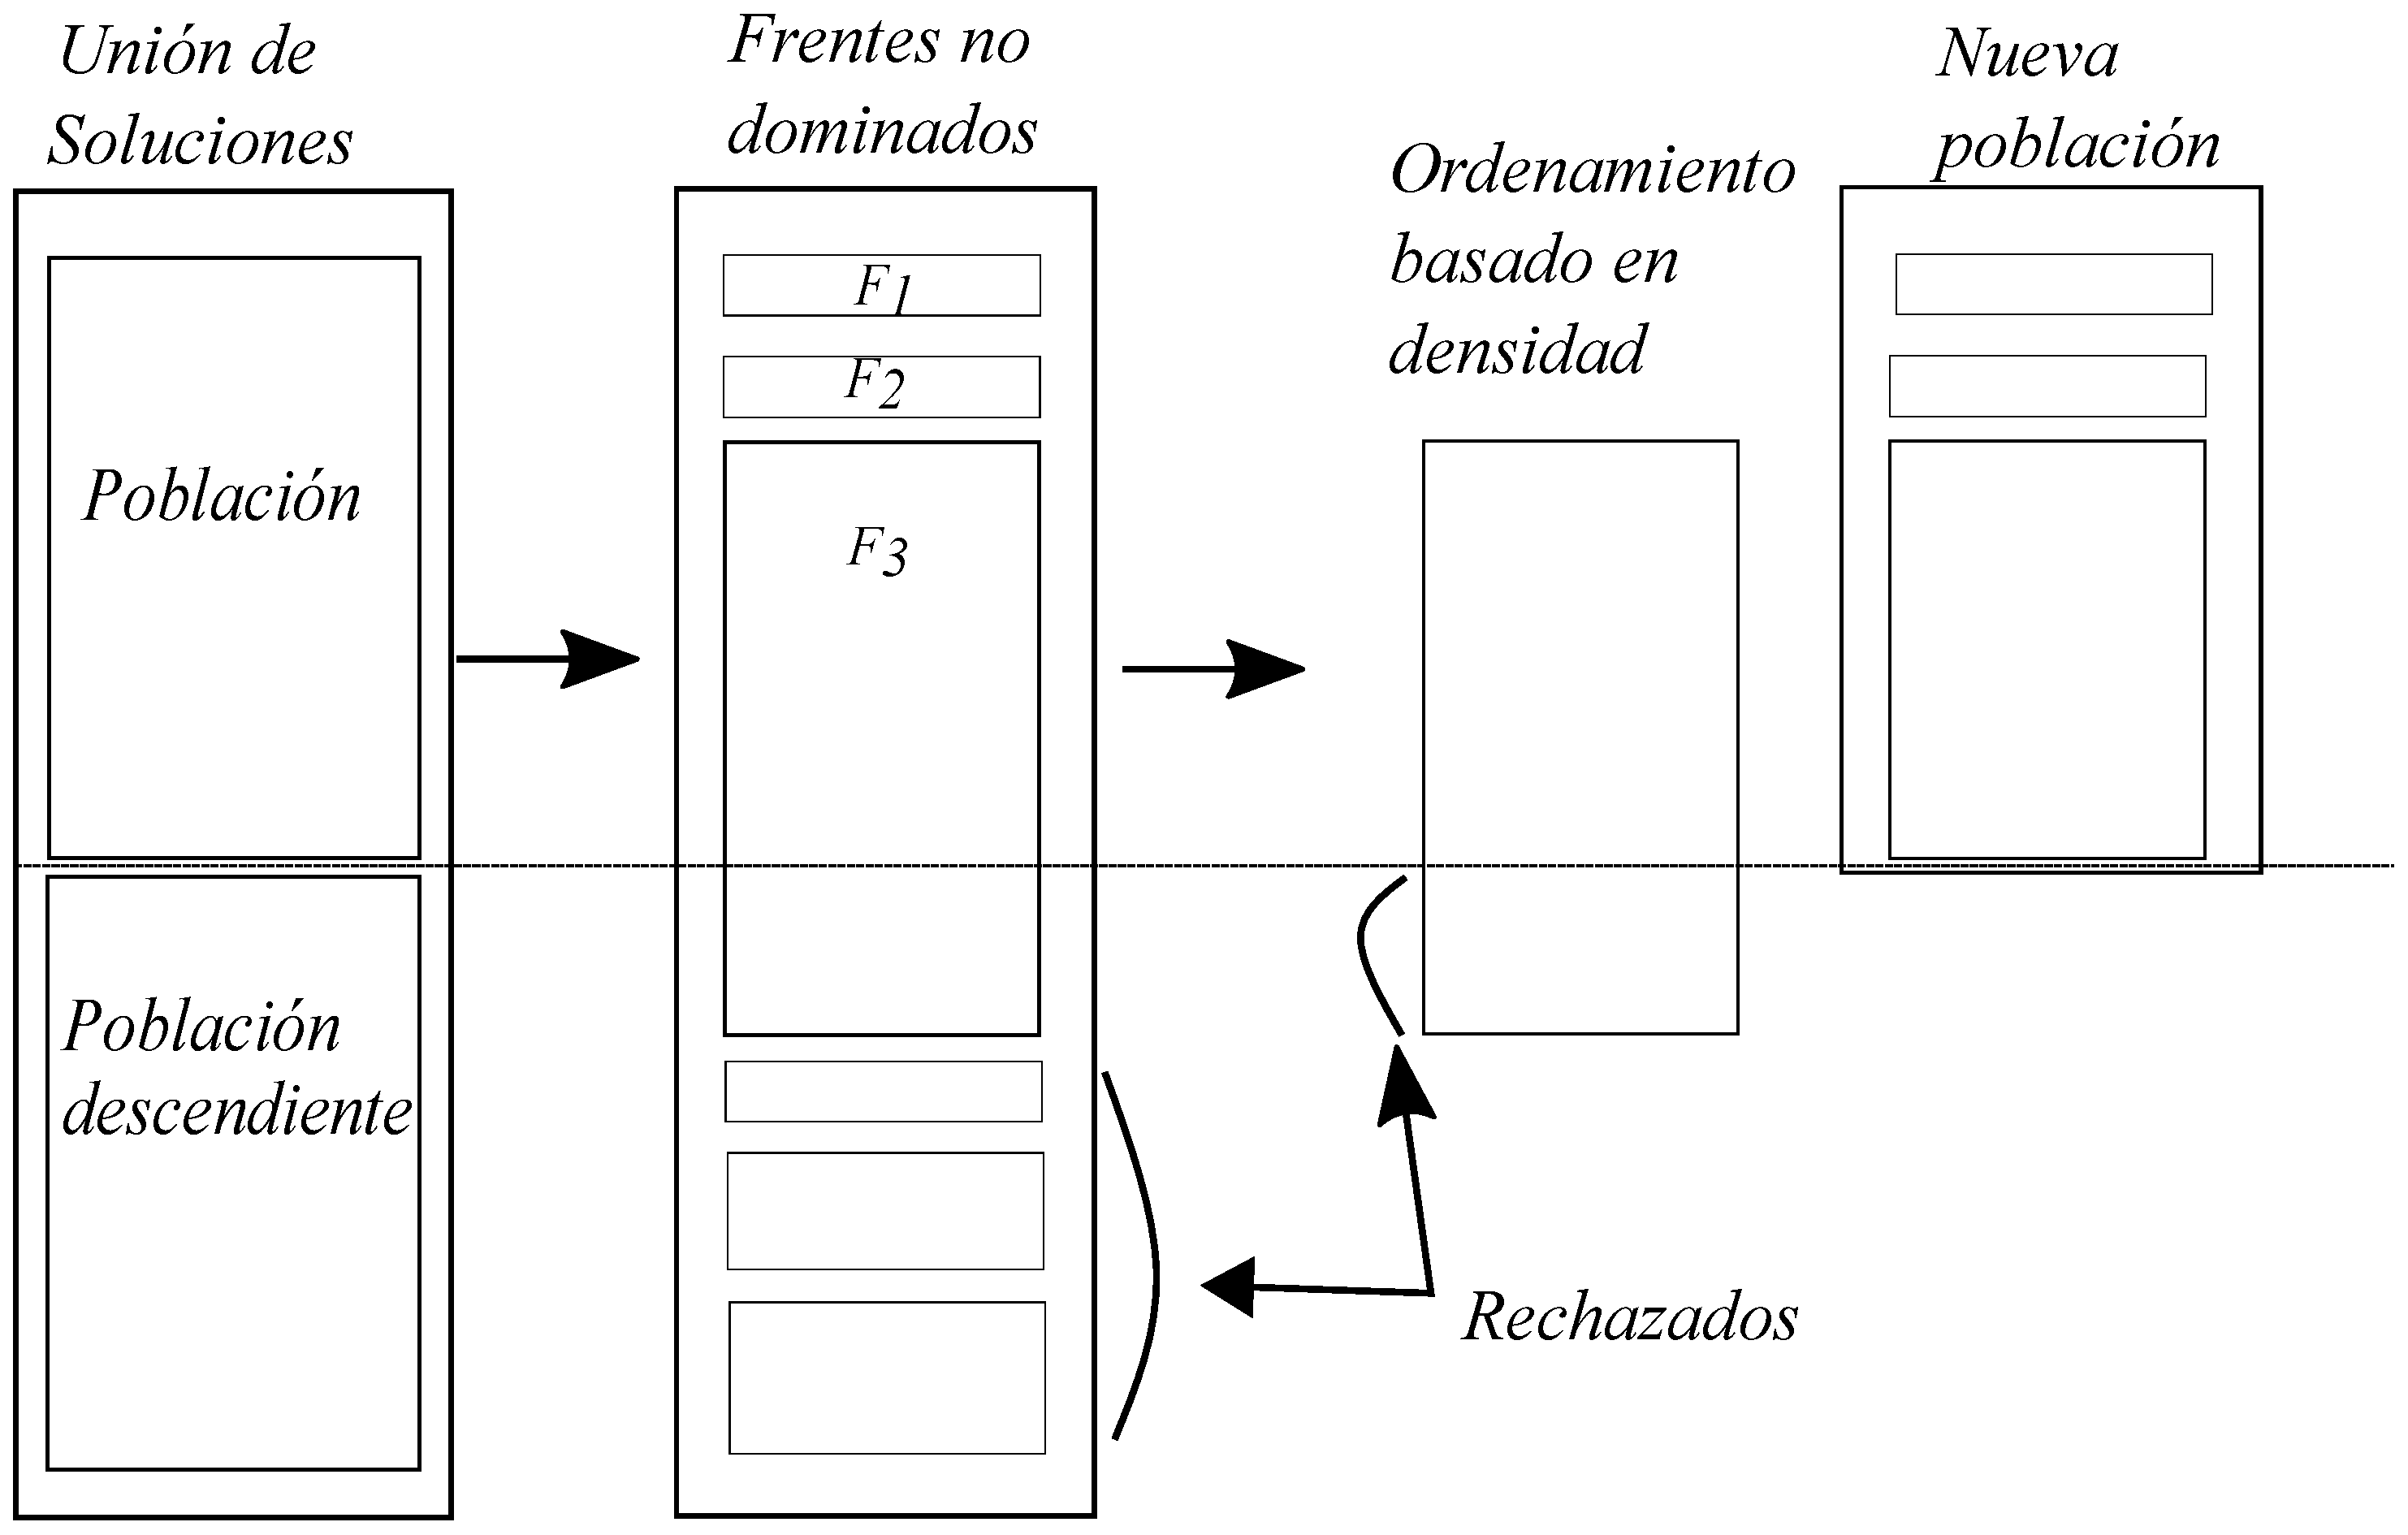
\includegraphics{Capitulo2/assets/ProcedimientoNSGAII.eps}
	\centering
	\caption[Procedimiento NSGAII]{Procedimiento NSGAII~\cite{Deb2002}}
	\label{fig:procedimientoNSGAII}
\end{figure}

A continuaci�n se proceder� a explicar los operadores adicionales presentados en~\cite{Deb2002} y que son utilizados por la funci�n de remplazo del algoritmo NSGAII en la Figura~\ref{fig:RemplaceNSGAII}.

\subsubsection{Ordenamiento de soluciones en frentes no dominados}
Uno de los procedimientos presentados en la Figura~\ref{fig:RemplaceNSGAII} consiste en ordenar las soluciones en frentes no dominados. Los frentes no dominados son conjuntos en los que se almacenan las soluciones que no se dominan entre si. En la Figura~\ref{fig:frente-no-dominados} se muestra un ejemplo con tres frentes.

\begin{figure}[h]
	 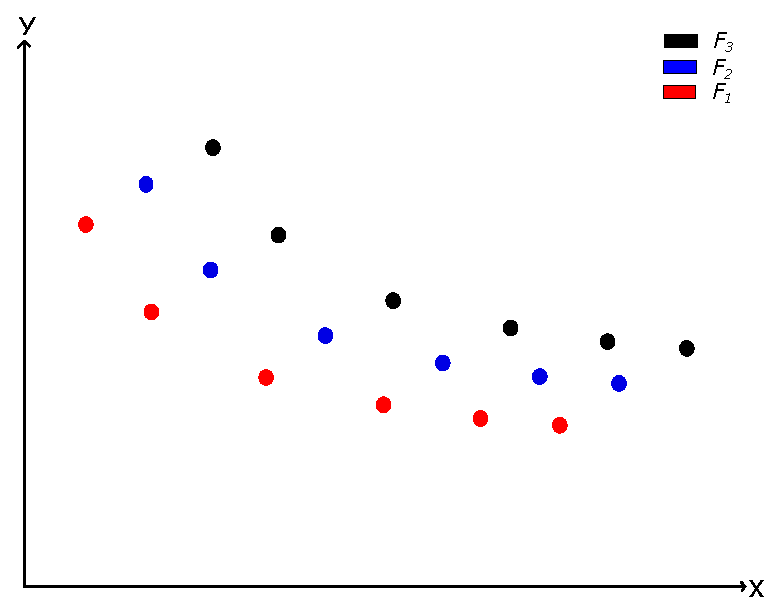
\includegraphics[scale=0.7]{Capitulo2/assets/frentes-no-dominados.eps}
	\centering
	\caption{Frentes no dominados}
	\label{fig:frente-no-dominados}
\end{figure}

El algoritmo para llevar a cabo esto se presenta en la Figura~\ref{fig:sortFront} y consiste en lo siguiente:

Primero, se debe comparar todas las soluciones entre si utilizando el concepto de dominancia de Pareto. Para ello, cada soluci�n $p$ cuenta con un atributo $S_p$ en el que guarda todas las soluciones a las que domina y un contador $n_p$ que almacena el numero de soluciones que lo dominan a �l. Cada vez que se termina de comparar una soluci�n con todas las otras, si su contador $n_p$ es igual a 0, se le asigna a la soluci�n el rango que indica el frente al que pertenece, y se guarda esta en un conjunto $F_1$ que contiene a todas las soluciones de dicho frente. 
	
Una vez que se han identificado todas las soluciones no dominadas del primer frente se procede a generar el siguiente, para lo cual, por cada soluci�n $q$ almacenada en el conjunto $S_p \in p$ del frente ya conocido, se disminuye en uno su contador $n_q$. Si el contador $n_q$ de la soluci�n $q$ llega a 0, entonces se le asigna a dicha soluci�n el rango correspondiente y se guarda esta en un conjunto temporal $Q$ con el resto de las soluciones en dicho frente. Cuando se tengan identificadas todas las soluciones, estas se asignan al frente correspondiente $F_i$. 

Finalmente, se repite el procedimiento anterior sobre el nuevo frente hasta haberlos generado todos.


\begin{figure}[h]
	\begin{algorithm}[H]
		\caption{Funci�n de ordenaci�n en frentes no dominados}
		\DontPrintSemicolon
		\SetKwData{PopulationVar}{poblaci�n}
		\SetKwData{Front}{$F$}
		\SetKwData{NewPopulation}{nuevaPoblacion}
		
		\SetKwFunction{FastNonDominatingSorting}{ordenarPorFrentesNoDominados}


		
		\SetKwProg{Fn}{Function}{}{fin}
		\Fn{\FastNonDominatingSorting(\PopulationVar)}{
		$\Front \leftarrow \emptyset$\;
		\tcc*[h]{Identificar el frente $F_1$}\;
		\ForEach{$p \in \PopulationVar$}{
			\tcc*[h]{Conjunto de soluciones dominadas por $p$}\;
			$S_p = \emptyset$\; 
			\tcc*[h]{Numeros de soluciones que dominan a $p$}\;
			$n_p = 0$\;
			\ForEach{$q \in \PopulationVar$}{
				\uIf(\tcc*[h]{$p$ domina a $q$}){$p \prec q$}{
					$S_p = S_p \cup \{q\}$\;
				}\ElseIf(\tcc*[h]{$q$ domina a $p$}){$q \prec p$}{
					$n_p = n_p + 1$\;
				}
				\If{$n_p = 0$}{
					$p_{rango} = 1$\;
					$F_1 = F_1 \cup \{p\}$\;
				}	
			}
		}
		\BlankLine
		$i = 1$\;
		\BlankLine
		\While{$F_i \neq \emptyset$}{
			$Q = \emptyset$\;
			\ForEach{$p \in \Front_i$}{
				\ForEach{$q \in S_p$}{
					$n_q = n_q - 1$\;
					\If{$n_q = 0$}{
						$q_{rango} = i + 1$\;
						$Q = Q \cup \{q\}$\;
					}
				}
			}

			$i = i+1$\;
			$F_i = Q$\;
		}
	}
		
	\end{algorithm}
	\caption[Pseudoc�digo de la funci�n de ordenamiento utilizada en NSGAII]{Pseudoc�digo de la funci�n de ordenamiento utilizada en NSGAII~\cite{Deb2002}}
	\label{fig:sortFront}
\end{figure}
\clearpage

\subsubsection{Densidad de estimaci�n (Crowing Distance)}
Otra funci�n presente en la Figura~\ref{fig:RemplaceNSGAII} es la asignaci�n de las densidades sobre cada soluci�n, la cual corresponde a la distancia promedio entre la soluci�n anterior y la siguiente a partir de cada uno de los objetivos. En la Figura~\ref{fig:crowdingDistance} la densidad de la soluci�n $i$ corresponde a la suma de la longitud del lado mayor y del lado menor del rect�ngulo.

\begin{figure}[H]
	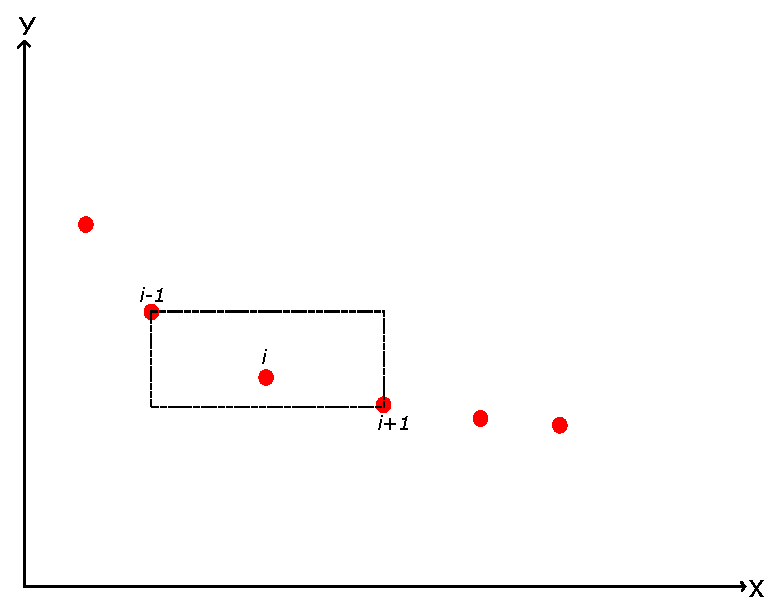
\includegraphics[scale=0.6]{Capitulo2/assets/crowing-distance.eps}
	\centering
	\caption[C�lculo de la densidad de estimaci�n al rededor de la soluci�n $i$]{C�lculo de la densidad de estimaci�n al rededor de la soluci�n $i$~\cite{Deb2002}}
	\label{fig:crowdingDistance}
\end{figure}

El procedimiento para esta funci�n  se muestra en la Figura~\ref{fig:crowdingDistance} y consiste en:

Primero, crear e inicializar un arreglo $\mathcal{I}_{distancia}$, con el valor 0, en donde guardar las distancias para cada soluci�n a medida que se van calculando. Luego, por cada uno de los objetivos se ordena el frente $\mathcal{I}$ y dentro $\mathcal{I}_{distancia}$ se le asigna al primer y ultimo elemento el valor infinito. Finalmente, se recorre desde la segunda hasta la pen�ltima soluci�n calculando la distancia $\mathcal{I}[i]_{distancia}$. Notar que $f_m^{max}$ y $f_m^{min}$ corresponden al valor del objetivo $m$ de la primera y �ltima soluci�n.

\begin{figure}[H]
	\begin{algorithm}[H]
	\caption{Funci�n de calculo de densidades}
	\DontPrintSemicolon
	\SetKwData{NDS}{$\mathcal{I}$}
	\SetKwFunction{CrowdingDistanceAssignament}{asignarDensidad}
		
		
		
	\SetKwProg{Fn}{Function}{}{fin}
	\Fn(\tcc*[h]{$\NDS$ : frente de soluciones no dominadas}){\CrowdingDistanceAssignament($\NDS$)}{
		$l = |\NDS|$ \tcc*[h]{Obtiene el tama�o del frente}\;\;
		\BlankLine
		\tcc*[h]{Inicializa la distancia para cada soluci�n}\;
		\ForEach{$i \leftarrow 1$ \KwTo $l$}{
			$\NDS[i]_{distancia} \leftarrow 0$
		}
		\ForEach{$m \leftarrow 1$ \KwTo numero de objetivos}{
			$\NDS \leftarrow$ sort($\NDS$, m) \tcc*[h]{Ordena por el objetivo m}\; 
			\BlankLine
			\tcc*[h]{Asignar a la primera y �ltima soluci�n el valor $\infty$ }\;
			$\NDS[1]_{distancia} \leftarrow \NDS[l]_{distancia} \leftarrow \infty$\;
			\BlankLine
			\For{$i \leftarrow 2$ \KwTo $l-1$}{
				\tcc*[h]{Asigna la distancia a las soluciones restantes}\;
				$\NDS[i]_{distancia} \leftarrow \NDS[i]_{distancia} + (\NDS[i+1].m - \NDS[i-1].m)/(f_m^{max} - f_m^{min})$\;	
			}
		}
	
	}
		
	\end{algorithm}
	\caption[Pseudoc�digo de la funci�n de asignaci�n de densidad]{Pseudoc�digo de la funci�n de asignaci�n de densidad~\cite{Deb2002}}
	\label{fig:CrowindDistance}
\end{figure}
\subsubsection{Comparador de densidad (Crowing Distance comparator)}
Este operador compara las soluciones basados en dos conceptos los cuales son el rango de dominaci�n y la densidad de soluciones. Estos fueron calculados al momento de generar los frentes y asignar la densidad a las soluciones. De acuerdo a Deb~\cite{Deb2002}, se define el orden dado por el operador de densidad ($\prec_n$) como: $i \prec_n j $, si $(i_{rango} < j_{rango})$ o $((i_{rango} = j_{rango})$ o $(i_{distancia} > j_{distancia}))$.
\newpage
\section{Problemas de optimizaci�n en RDA}
Basado en los requisitos se han seleccionado dos problemas; optimizaci�n del dise�o de RDA basado en la selecci�n del di�metro de tuber�as (\textit{Pipe Optimizing}) y la optimizaci�n del r�gimen de bombeo (\textit{Pumping Schedule}). Y en esta secci�n se representan sus modelos matem�ticos asi como la codificaci�n implementada.

\subsection{\textit{Pipe Optimizing}}
\textit{Pipe Optimizing} es un problema de dise�o cuyo objetivo es minimizar el costo de inversi�n en la construcci�n de las tuber�as. Para �sto, se busca aquella combinaci�n de di�metros que disminuyan el costo de la construcci�n de las tuber�as a la vez que se cumplen las restricci�n de presi�n m�nima impuesta sobre la red. La ecuaci�n \ref{eq:costos_de_inversion} presentada en \cite{Pereyra2017} muestra la ecuaci�n a optimizar.
	
\begin{equation}
    \label{eq:costos_de_inversion}
    \begin{aligned}
        \text{Costo de inversi�n} = \sum_{i=1}^{N} (C_i \times D_i \times L_i)
    \end{aligned}
\end{equation}

En la ecuaci�n anteriormente presentada el termino $C_i$ se refiere al costo unitario de la tuber�a $i$, el t�rmino $D_i$ corresponde al di�metro de la tuber�a y finalmente $L_i$ hace referencia su longitud. Como se mencion� anteriormente, el problema debe satisfacer la siguiente restricci�n:

\begin{equation}
    \label{eq:restriccion_costo_inversion}
    \begin{aligned}
        H_i < H_{min}
    \end{aligned}
\end{equation}

\noindent donde $H_i$ corresponde a la presi�n sobre la tuber�a $i$ y $H_{min}$ a la presi�n m�nima de la red.

La soluci�n retornada por el algoritmo utilizado, en este caso GA, se puede ver en la Figura~\ref{fig:solution_pipe_optimizing}. En dicha soluci�n los valores que toman la variable de decisi�n corresponden al �ndice a una tabla donde se encuentra el di�metro y el costo de la tuber�a. El largo de la tuber�a esta configurado en el archivo de configuraci�n de red (El archivo con extensi�n inp). 

\begin{figure}[H]
    \centering
    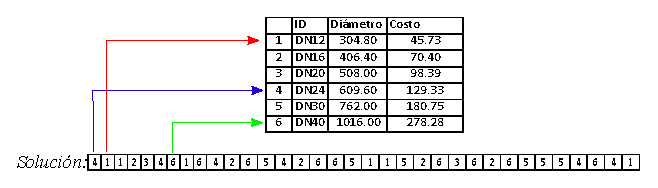
\includegraphics[width=\textwidth]{Capitulo2/assets/representacion_solucion_monoobjetivo.eps}
    \caption{Representaci�n de la soluci�n del problema monoobjetivo \textit{Pipe Optimizing}}
    \label{fig:solution_pipe_optimizing}
\end{figure}

\subsection{\textit{Pumping Schedule}}

\textit{Pumping Schedule} \cite{Makaremi2017, JHawanet-2019} es un problema de operaci�n que tiene como objetivos optimizar tanto el costo energ�tico, as� como el costo de mantenci�n de los equipos de bombeos. A continuaci�n se expresan las ecuaciones utilizadas para calcular los objetivos y las restricciones.

Para el c�lculo de los costos energ�ticos se ocupa la siguiente ecuaci�n:
  
\begin{equation}
    \label{eq:costos_energeticos}
    \begin{aligned}
        C_E(S) &= \sum_{n=1}^{NP}\sum_{t=0}^{NT-1}(P_c(t) \times E_c(n, t) \times S(n, t))
    \end{aligned}
\end{equation}

\noindent donde:
\begin{itemize}
    \item	$C_E(S)$: Costos energ�tico.
    \item   $NP$: El numero de bombas.
    \item 	$NT$: N�mero de periodos de simulaci�n. El m�ximo son 24 horas.
    \item 	$P_c(t)$: La tarifa energ�tica en el periodo $t$.
    \item 	$E_c(n, t)$: Consumo energ�tico de la bomba $n$ en el tiempo $t$.
    \item 	$S(n,t)$: El estado de la bomba. 1 si esta encendida y 0 si esta apagada.
\end{itemize}

Para calcular el consumo energ�tico de la bomba $n$ se utiliza la siguiente formula:
\begin{equation}
    \label{eq:costos_energeticos}
    \begin{aligned}
        E_c(n, t) &= \frac{10^{-3} \times \gamma \times Q(n, t) \times h(n, t)}{e(n, t)}
    \end{aligned}
\end{equation}

\noindent donde:
\begin{itemize}
    \item	$\gamma$: Peso del agua.
    \item   $Q(n, t)$: Flujo a trav�s de la bomba $n$ en el tiempo $t$
    \item 	$h(n, t)$: Altura manom�trica de la bomba.
    \item 	$e(n, t)$: Eficiencia de la bomba $n$ en el tiempo $t$.
\end{itemize}

Para c�lcular el costo de mantenimiento se c�lcula el n�mero de encendido y apagados de todas las bombas en el periodo de tiempo analizado. Matem�ticamente la funci�n para calcular dicho costo corresponde a:

\begin{equation}
    \label{eq:costos_de_mantenimiento}
    \begin{aligned}
        C_N(S) &= \sum_{n=1}^{NP}\sum_{t=0}^{NT-1}r_t
    \end{aligned}
\end{equation}
donde:
\begin{itemize}
    \item $C_N(S)$: Costo de mantenimiento.
    \item $r_t$: Valor indicando si en el periodo $t$ hubo un cambio de estado en la bomba desde apagado a encendido. Este valor es 1 cuando la bomba ha sido encendida.
\end{itemize}

La funciones \ref{eq:costos_energeticos} y \ref{eq:costos_de_mantenimiento} deben cumplir las siguientes restricciones:
% restricciones asociadas a la conservaci�n de la masa y la energ�a; la presi�n m�nima, el caudal en la bomba $n$ y el nivel de agua almacenado en el reservorio en un periodo de tiempo especifico.

Conservaci�n de la masa:
\begin{equation}
    \label{eq:conservation_of_mass}
    \begin{aligned}
        \sum q_{in}-q_{out} &= C_j
    \end{aligned}
\end{equation}

\noindent donde:
\begin{itemize}
    \item $q_{in}$: Flujo de entrada.
    \item $q_{out}$: Flujo de salida.
    \item $C_j$: Consumo del nodo $j$.
\end{itemize}

Conservaci�n de la energ�a:
\begin{equation}
    \label{eq:conservation_of_energy}
    \begin{aligned}
        \sum h_f - \sum E_p &= 0
    \end{aligned}
\end{equation}

\noindent donde:
\begin{itemize}
    \item $h_f$: Perdida de energ�a por fricci�n.
    \item $E_p$: Energ�a aportada por la bomba.
\end{itemize}

Perdida de carga por fricci�n:
\begin{equation}
    \label{eq:pipe_head_losses}
    \begin{aligned}
        h_f &= \frac{10.67 \times L_q^{1.85}}{CH^{1.85} \times D^{4.87}}
    \end{aligned}
\end{equation}

\noindent donde:
\begin{itemize}
    \item $L_q$: Largo de la tuber�a.
    \item $CH$: Coeficiente de Hazen-Williams.
    \item $D$: Di�metro de la tuber�a.
\end{itemize}

Presi�n m�nima:
\begin{equation}
    \label{eq:min_pressure}
    \begin{aligned}
        H_i < H_{min}
    \end{aligned}
\end{equation}

\noindent donde:
\begin{itemize}
    \item $H_i$: Presi�n en el nodo $i$.
    \item $H_{min}$: Presi�n m�nima.
\end{itemize}

Caudal:
\begin{equation}
    \label{eq:min_pressure}
    \begin{aligned}
        Q_{i,t} \geq Q_i^{max}
    \end{aligned}
\end{equation}

\noindent donde:
\begin{itemize}
    \item $Q_{i,t}$: Caudal del nodo $i$ en el tiempo $t$.
    \item $Q_i^{max}$: Caudal m�ximo del nodo $i$.
\end{itemize}

Nivel de dep�sito:
\begin{equation}
    \label{eq:min_pressure}
    \begin{aligned}
        TS_{i, NT} \geq TS_{i, 0}
    \end{aligned}
\end{equation}

\noindent donde:
\begin{itemize}
    \item $TS_{i, NT}$: Nivel del reservorio $i$ en el tiempo $t$.
    \item $TS_{i, 0}$: Nivel del reservorio $i$ en el tiempo $0$.
\end{itemize}

En la Figura~\ref{fig:solution_pump_schedule} muestra como se codifica la soluci�n a este problema propuesta por~\cite{JHawanet-2019}. Como se puede observar la soluci�n cuenta con 24 variables de decisi�n correspondiente a las 24 horas del d�a. Cada variable es un �ndice a la matriz de combinaciones posibles para cada bomba. Posteriormente, se genera una matriz binaria en donde cada fila es una bomba, cada columna es el periodo y el valor es el estado de la bomba en dicho periodo. Esta matriz binaria es usada para calcular el n�mero de cambios de estado en las bombas de la ecuaci�n \ref{eq:costos_de_mantenimiento}, asi como para obtener el estado de la bomba en el periodo $t$ de la ecuaci�n \ref{eq:costos_energeticos} referente al termino $S(n, t)$.

\begin{figure}[H]
    \centering
    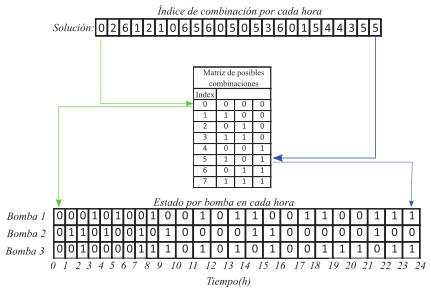
\includegraphics[width=\textwidth]{Capitulo2/assets/representacion_solucion_multiobjetivo.eps}
    \caption{Representaci�n de la soluci�n problema multiobjetivo \textit{Pumping Schedule}}
    \label{fig:solution_pump_schedule}
  \end{figure}
\section{Trabajo relacionado}
En este apartado se mostrar�n distintas herramientas y el enfoque utilizado para resolver el problema con ellas. En general, los enfoques consisten en usar software ya disponible o crear un software personalizado.

\begin{itemize}
	\item \textbf{Magmoredes}: En~\cite{Edwin2017} se describe la existencia de un software de dise�o basado en micro-algoritmos gen�ticos multiobjetivos, que de acuerdo al autor, tiene un mejor rendimiento y es m�s eficiente que el algoritmo NSGAII. Esto se debe a que requiere una menor cantidad de memoria y tiene un mejor tiempo de c�mputo. Este programa puede cargar cualquier red y realiza los c�lculos utilizando librer�as de Java. Las funciones objetivos que este sistema intenta resolver son la optimizaci�n de los costos de construcci�n de la red y la confiabilidad final de la red.
	
	\item \textbf{WaterGEMS}: Software comercial que permite la construcci�n de modelos geoespaciales; optimizaci�n de dise�o, ciclos de bombeo y calibraci�n autom�tica del modelo; y la gesti�n de activos. Este software a sido usado en~\cite{Mehta2017} para llevar a cabo las simulaciones necesarias para su estudio. La metodolog�a seguida para la utilizaci�n de este sistema consiste en ingresar los datos a WaterGEMS para correr las simulaciones. La limitaci�n de este programa es que no permite la adici�n de nuevos algoritmos por parte del usuario, en el caso de que se quiera probar o mejorar alg�n algoritmo ya existente. Sin embargo, este sistema tambi�n tiene sus ventajas, porque ya incorpora algunos algoritmos predefinidos para resolver ciertos problemas. Adem�s, posee diversas funcionalidades como conexi�n con datos externos, operaciones de an�lisis espaciales, intercambio de datos con dispositivos o programas de administraci�n, entre otros.
	
	\item \textbf{EPANET}: El enfoque seguido con la utilizaci�n de esta herramienta consiste en automatizar la ejecuci�n de los algoritmos y la posterior evaluaci�n de los resultados utilizando la librer�a EPANET Toolkit. Este es usado en~\cite{Doctoral2012} en donde se implementan ciertos algoritmos metaheur�sticos y los resultados obtenidos por estos son enviados a la EPANET Toolkit para evaluar la soluci�n y determinar la factibilidad de �sta. La ventaja de este enfoque es que permite una mayor flexibilidad en los algoritmos metaheuristicos utilizados y los problemas que se quieren resolver. Sin embargo, debido a que se necesita implementar los problemas y los algoritmos, este enfoque toma mucho tiempo.
\end{itemize}

Para el desarrollo de este proyecto se usa el enfoque basado en EPANET, puesto que es una librer�a de simulaci�n hidr�ulica ampliamente utilizada y permite enfocarnos en la resoluci�n de los problemas usando algoritmos metaheur�sticos. Tanto Magmoredes como WaterGEMS buscan resolver temas concretos en los sistemas de distribuci�n de agua potable y puesto que el c�digo de estos programas no esta disponible p�blicamente o son un sistema que se comercializa sin permitir la modificaci�n del sistema por parte de terceros, se busca con nuestro proyecto incorporar esta capacidad para que en futuros trabajos se pueda abarcar una mayor cantidad de problemas en nuestro sistema.

\chapter{Metodolog�a de desarrollo}
En este cap�tulo se presenta la metodolog�a a seguir durante el desarrollo del proyecto, as� como las fases que la componen y las tareas que son realizadas por cada una de estas fases.

La metodolog�a escogida para utilizar durante el desarrollo de este proyecto es la metodolog�a iterativa e incremental.

Debido a que la metodolog�a esta pensada para ser llevada a cabo por un equipo de trabajo, esta se ha adaptado para poder ser aplicada en el desarrollo llevado a cabo por una sola persona. Esta adaptaci�n puede ser resumida en los siguientes puntos:
\begin{itemize}
	\item Disminuye la cantidad de documentaci�n generada por cada fase.
	\item Permite llevar a cabo m�s de una fase dentro de cada iteraci�n al mismo tiempo.
	\item Los roles de analista, dise�ador, implementador y tester son realizados por una sola persona.
\end{itemize}

Las tareas a desempe�ar por cada fase consisten en:
\paragraph{An�lisis:}
\begin{itemize}
	\item \textbf{Captura de requisitos:} durante esta etapa se realiza una reuni�n con el cliente ya sea f�sica o remotamente, se conversa y llega a un acuerdo acerca de las funcionalidades que deben ser implementadas en la aplicaci�n.
	\item \textbf{Priorizaci�n de los requisitos:} junto con el interesado se le asigna una prioridad a los requisitos capturados con el fin de establecer el orden en que estos deben ser implementados.
	% \item Validaci�n de requisitos.
	\item \textbf{Especificaci�n formal de requisitos:} en esta etapa se redacta un documento aparte donde se especifican de manera formal los requisitos. La especificaci�n contiene los siguientes datos por cada uno de los requisitos identificados: id del requisito, descripci�n, fuente, prioridad, estabilidad, fecha de actualizaci�n, estado de la implementaci�n, incremento y el tipo de requisito.
\end{itemize}
\paragraph{Dise�o:} 
\begin{itemize}
	\item \textbf{Definici�n y especificaci�n de la arquitectura del sistema:} durante esta etapa se especifica tanto la arquitectura f�sica como l�gica de la aplicaci�n.
	\item \textbf{Dise�o de las interfaces de usuario:} se dise�an las interfaces de usuario de la aplicaci�n. Este dise�o se realiza utilizando herramientas de \textit{mockup}, implementando las interfaces directamente sin funcionalidad.
	\item D\textbf{ise�o de los componentes:} se realiza un diagrama de los componentes que conforman la aplicaci�n.
	\item \textbf{Especificaci�n formal del dise�o del sistema:} se redacta un documento en el que se presentan los diagramas, las interfaces y los detalles de la implementaci�n.
\end{itemize}
\paragraph{Implementaci�n:}
\begin{itemize}
	\item \textbf{Programaci�n de los componentes de software:} implementaci�n de las funcionalidades para cumplir con los requisitos.
	\item \textbf{Integraci�n de los componentes de software:} consiste en tomar cada uno de los m�dulos independientes e integrarlos dentro de un solo sistema.
	\item \textbf{Elaboraci�n del producto entregable:} se empaqueta la aplicaci�n para generar un archivo que pueda ser distribuido. �ste, puede ser un archivo con extensi�n .jar o generar una aplicaci�n que posea todas las dependencies, incluyendo Java, y que se ejecuta a partir del archivo de extensi�n exe.
	\item \textbf{Elaboraci�n de manual de usuario:} consiste en redactar un manual de usuario que indica como realizar las tareas dentro de la aplicaci�n.
\end{itemize}
\paragraph{Pruebas:}
\begin{itemize}
	\item \textbf{Definici�n de casos de prueba:} esta tarea consiste en identificar las pruebas que deben ser realizadas para validar los componentes del sistema. Se dividen en dos tipos de prueba; automatizadas y manuales.
	\item \textbf{Especificaci�n formal de pruebas:} se redacta un documento en donde se especifican las pruebas realizadas. Para cada especificaci�n de los caso de prueba se definen los siguientes elementos: id de prueba, t�tulo, caracter�stica a evaluar, el objetivo de la evaluaci�n, la configuraci�n de la aplicaci�n al momento de realizar la prueba, los datos de prueba, las acciones que hay que realizar durante la prueba y finalmente los resultados esperados de la ejecuci�n.
	\item \textbf{Ejecuci�n de pruebas:} durante esta etapa se ejecutan las pruebas sobre el programa y se documenta los errores encontrados para ser resueltos en la iteraci�n posterior, si es que son complejos de resolver. Si los errores encontrados son simples se resuelven en el momento.
	% \item Validaci�n del producto.
	% \item Registro de incidencias.
\end{itemize}

Cada una de las fases mencionadas anteriormente tiene como resultado un documento de especificaci�n formal con el siguiente contenido:

\paragraph{Especificaci�n formal de requisitos:}
\begin{itemize}
	\item \textbf{Introducci�n:} En este apartado del documento se da una introducci�n al problema que se ha identificado.
	\item \textbf{Requisitos de usuario:} Consiste en la recopilaci�n de lo requisitos de los usuarios que deben ser cumplidos al final del periodo de desarrollo.
	\item \textbf{Requisito de sistema:} Son los requisitos, desde un punto de vista mas t�cnico, que son necesarios para satisfacer los requisitos de usuario.
	\item \textbf{Matriz de trazado requisitos de usuario versus sistema:} Matriz que permite ver la trazabilidad de los requisitos de usuario con los de sistema.
\end{itemize}
\paragraph{Especificaci�n formal del dise�o del sistema:}
\begin{itemize}
	\item \textbf{Casos de uso:} Serie de diagramas que permiten ver la interacci�n que el usuario tiene con el sistema.
	\item \textbf{Arquitectura f�sica:} Descripci�n de los componentes f�sicos que intervienen en la aplicaci�n.
	\item \textbf{Arquitectura l�gica:} Descripci�n a alto nivel del software y los componentes que lo componen.
	\item \textbf{Diagrama de componentes:} Permite ver la divisi�n del sistema y la interacci�n entre los distintos componentes~\cite{Bell2004}.
	\item \textbf{Dise�o de interfaces:} Bosquejos o implementaci�nes de las interfaces a ser utilizadas en la propuesta.
	\item \textbf{Diagrama de clases:} Describe la relaci�n entre las distintas clases presentes en la soluci�n propuesta.
\end{itemize}
\paragraph{Manual de usuario:} Explicaci�n acerca de las capacidades de la aplicaci�n, acompa�ada de esquemas y ejemplos de uso.
\paragraph{Especificaci�n formal de pruebas:}  Se documenta las pruebas automatizadas y manuales que se realizan y sobre que elemento se llevan a cabo.

La raz�n por la que se utiliza esta metodolog�a sobre otras es porque el producto resultante de este proyecto esta pensado para servir como base para futuros trabajos. Debido a esto, es necesario documentar detalladamente la implementaci�n para que otros programadores puedan continuar con su desarrollo en el futuro. Aunque existen otras metodolog�as como Cascada u otras tradicionales, estas son dif�ciles de llevar a cabo por la cantidad de documentaci�n que se requiere, mientras que metodolog�as de desarrollo �gil carecen en cuanto a la documentaci�n que se necesita para el sistema a desarrollar. Adicionalmente, esta metodolog�a nos permite obtener una retroalimentaci�n al final de cada iteraci�n, obtener nuevos requisitos que no hayan quedado definidos en etapas anteriores o refinar los requisitos y el dise�o ya existente, permitiendo as� mejorar la calidad del producto final.

La implementaci�n de esta metodolog�a para el desarrollo del proyecto se lleva a cabo repartiendo las tareas necesarias para el cumplimiento de los objetivos en iteraciones. De este modo al final de cada iteraci�n se cuenta con un prototipo funcional de la aplicaci�n sobre el que se agrega las nuevas funcionalidades en las iteraciones siguientes.

\chapter{Desarrollo}
En esta cap�tulo se da a conocer la concepci�n del proyecto, la planificaci�n de las iteraciones y se detalla como se aplica la metodolog�a en el desarrollo del proyecto. Para esto, se presenta por cada una de las fases del desarrollo las actividades realizadas en cada iteraci�n utilizando una serie de casos de prueba a modo de ejemplos de las funcionalidades a implementar. 

\section{Concepci�n del proyecto}

Este proyecto se origina como una propuesta por parte del profesor del departamento de Ingenier�a en Obras Civiles, Daniel Mora Melia. �l, junto a un grupo de expertos de diversas �reas, presentaron y publicaron un articulo del proyecto JHawanet~\cite{JHawanet-2019}. Dicho articulo, presenta la integraci�n de dos librer�as independientes, JMetal y Epanet, como herramienta para llevar a cabo optimizaciones sobre RDA. JMetal~\cite{Durillo2010} es un Framework de Java, orientado a la optimizaci�n multiobjetivo y es usado como motor de optimizaci�n. Mientras que Epanet~\cite{Rossman1999} es una herramienta la cual permite realizar simulaciones en redes de agua potable.

Debido al articulo anteriormente mencionado, surgi� la idea de crear una herramienta gr�fica con el fin de facilitar la optimizaci�n de redes de agua potable. Puesto que la utilizaci�n de la herramienta JHawanet requiere conocimiento computacional avanzado. Y de esta forma, permitir el trabajo de Ingenieros hidr�ulicos en un entorno especialmente dise�ado para su �rea sin perder la capacidad que la herramienta posee para que usuarios avanzados puedan incorporar y evaluar nuevos problemas y algoritmos. 


\section{Casos de prueba}

Los casos de prueba son las funcionalidades que se usar�n para presentar y demostrar la aplicaci�n de la metodolog�a durante el desarrollo del proyecto.

Se escoger�n 3 funcionalidades de prueba las cuales son:

\paragraph{Funcionalidad 1:} El sistema debe poder visualizar la red.

Esta funcionalidad consiste en visualizar gr�ficamente la forma de la red cargada. El archivo de descripci�n de red debe ser creado desde la aplicaci�n Epanet y tener la extensi�n inp.

\paragraph{Funcionalidad 2:} El sistema debe poder buscar soluciones al problema de la optimizaci�n de los costos de construcci�n de las tuber�as usando el algoritmo gen�tico.

Esta funcionalidad consiste en buscar soluciones para el problema de optimizaci�n de los costos de construcci�n de las tuber�as.

\paragraph{Funcionalidad 3:}  El sistema debe poder realizar una simulaci�n hidr�ulica utilizando los valores por defecto del archivo de red.

Esta funcionalidad consiste en realizar una simulaci�n hidr�ulica utilizando el archivo de red cargado y visualizar los valores resultantes de los elementos de la red.
\section{Planificaci�n}

Como se menciono en la secci�n anterior, para llevar a cabo el desarrollo del proyecto se opto por la metodolog�a iterativa e incremental. La planificaci�n resultante seguida durante el desarrollo del proyecto se muestra en el Cuadro \ref{fig:planificacion}.

\begin{table}
  \begin{center}
    \caption{Planificaci�n de las iteraciones}
    \begin{tabular}{||c| m{6cm}| m{2.5cm}| m{2.5cm}||} 
      \hline
      N� Iteraci�n & Tareas & Fecha Inicio & Fecha \newline t�rmino \\ [0.5ex] 
      \hline\hline
      1 & - Especificaci�n de requisitos \newline - Escoger arquitectura l�gica y f�sica & 26/08/2019 & 14/10/2019 \\ 
      \hline
      2 & - Implementar problema monoobjetivo (Pipe Optimizing) \newline - Implementar algoritmo gen�tico \newline - Implementar operadores de selecci�n y reproducci�n & 14/10/2019 & 11/11/2019 \\
      \hline
      3 & - Crear interfaces de usuario \newline - Guardar soluciones & 11/11/2019 & 20/01/2020 \\
      \hline
      4 & - Implementar problema multiobjetivo (Pumping Scheduling) \newline - Implementar algoritmo NSGAII & 27/01/2020 & 24/02/2020 \\
      \hline
      5 & - Permitir realizar m�ltiples repeticiones de un algoritmo \newline - Permitir realizar la simulaci�n usando los valores por defecto de la red & 02/03/2020 & 04/05/2020 \\ [1ex] 
      \hline
      6 & - Agregar s�mbolos al dibujo de la red \newline - Exportar a excel \newline - Agregar menu de configuraci�n & 11/05/2020 & 08/06/2020 \\ [1ex] 
      \hline
    \end{tabular}
   \label{fig:planificacion}
 \end{center}
\end{table}
\section{Requisitos}

Durante la fase de requisitos se llevo a cabo la captura, priorizaci�n, validaci�n y la especificaci�n formal de requisitos.

Los requisitos iniciales de la aplicaci�n fueron capturados del profesor Jimmy Gutierrez. Posteriormente, estos requisitos fueron priorizados y validados para finalmente ser documentados en el documento de especificaci�n formal de requisitos. 

A medida que avanzaban las iteraci�nes algunos requisitos fueron cambiando o fueron surgiendo requisitos nuevos. En el Cuadro~\ref{fig:cambios_requisitos} se detallan los cambios y actividades realizados durante cada iteraci�n.

\begin{table}
  \begin{center}
    \caption{Actividades y cambios de la fase de requisitos durante cada iteraci�n}
    \bigskip
    \begin{tabular}{||c| m{2cm}| m{8cm}||} 
      \hline
      N� Iteraci�n & Requisitos cubiertos & Tareas\\ [0.5ex] 
      \hline\hline
      1 & 5/32 & Se capturan 5 requisitos.\newline Se crea el informe de especificaci�n de requisitos. \\
      \hline
      2 & 11/32 & Se capturan 6 nuevos requisitos. \newline Se actualiza el documento de requisitos.\\
      \hline
      3 & 16/32 & Se capturan 5 nuevos requisitos. \newline Se actualiza el documento de requisitos. \\
      \hline
      4 & 20/32 & Se capturan 4 nuevos requisitos.\newline Se actualiza el documento de requisitos. \\
      \hline
      5 & 20/32 & No hay nuevos requisitos. \\
      \hline
      6 & 32/32 & Se capturan 12 nuevos requisitos.\newline Se actualiza el documento de requisitos. \\
      \hline

    \end{tabular}
   \label{fig:cambios_requisitos}
 \end{center}
\end{table}

Los cuadros~\ref{fig:RU004},~\ref{fig:RU002} y~\ref{fig:RU020} muestran la especificaci�n formal de los requisitos relacionados a las funcionalidades escogidas anteriormente.

\begin{requisito}[fig:RU004][Especificaci�n del requisito de usuario RU004.]
  \Requisito{RU004}{Visualizar red en una interfaz gr�fica.}
  \Descripcion{Se debe mostrar en la interfaz gr�fica una representaci�n de la red (Un dibujo, etc) generada a partir de la informaci�n contenida en el archivo inp.}
  
  \Fuente{Jimmy Guti�rrez}
  \Prioridad{Cr�tica}
  \Estabilidad{Intransable}
  \FechaA{09/09/2019}
  \Estado{Cumple}
  \Incremento{3}
  \Tipo{Funcional}
\end{requisito}

\begin{requisito}[fig:RU002][Especificaci�n del requisito de usuario RU002.]
  \Requisito{RU002}{Resolver el problema monoobjetivo (Pipe Optimizing)  usando el Algoritmo Gen�tico.}
  \Descripcion{El algoritmo gen�tico debe ser aplicado para resolver el problema monoobjetivo que tiene como funci�n objetivo el costo de inversi�n y como variable de decisi�n el di�metro de las tuber�as.}
  
  \Fuente{Jimmy Guti�rrez}
  \Prioridad{Cr�tica}
  \Estabilidad{Intransable}
  \FechaA{09/09/2019}
  \Estado{Cumple}
  \Incremento{2}
  \Tipo{Funcional}
\end{requisito}

\begin{requisito}[fig:RU020][Especificaci�n del requisito de usuario RU020.]
  \Requisito{RU020}{Permitir realizar simulaciones hidr�ulicas utilizando los valores por defectos que vienen en el archivo .inp y visualizar los resultados.}
  \Descripcion{Utilizando los valores que vienen por defecto en el archivo inp se debe poder llevar a cabo la simulaci�n hidr�ulica de la red. Posteriormente, los resultados podr�n ser visualizados por el usuario.}
  
  \Fuente{Daniel Mora-Meli�}
  \Prioridad{Cr�tica}
  \Estabilidad{Intransable}
  \FechaA{27/01/2020}
  \Estado{Cumple}
  \Incremento{5}
  \Tipo{Funcional}
\end{requisito}

La especificaci�n formal de los requisitos restantes se encuentra en el \textbf{Anexo~\ref{appendix:requisito}}.






\section{Dise�o}

Una vez terminada la fase de requisitos se procede a dise�ar la aplicaci�n. Dentro del dise�o, se encuentran las tareas de escoger  y documentar la arquitectura f�sica y l�gica, realizar los diagramas de clases, diagramas de secuencia, dise�o de interfaces, entre otros.

Mientras avanzaba el desarrollo fue necesario ir modificando el documento de dise�o debido a la aparici�n o al cambio de requisitos, as� como la realizaci�n de mejoras en los diagramas realizados. En el Cuadro \ref{fig:cambios_diseno} se presentan m�s detalladamente los cambios realizados en cada iteraci�n.

\begin{table}
  \begin{center}
    \caption{Actividades y cambios de la fase de requisitos durante cada iteraci�n}
    \begin{tabular}{||c| m{6cm}| m{6cm}||} 
      \hline
      N� Iteraci�n & Tareas & Comentario\\ [0.5ex] 
      \hline\hline
      1 & Crear arquitectura l�gica. \newline Crear arquitectura f�sica. \newline Dise�ar m�dulos.\newline Crear diagrama de clases del modulo metaheur�stica. \newline Crear diagrama de clases del la representaci�n de la red.
      & Durante esta iteraci�n se creo el documento de dise�o y se crearon los esquemas b�sicos para orientar la construcci�n del software.\\
      \hline
      2 & No hubieron cambios & No hubieron cambios en esta iteraci�n en el aspecto del dise�o.\\
      \hline
      3 & Dise�ar interfaces de usuario.\newline Especificar detalles de la implementaci�n referente a las anotaciones de java (Java Annotations).\newline Generar diagrama de secuencia de optimizaci�n. & Durante esta fase de dise�aron algunas de las interfaces de usuario de la aplicaci�n. \newline Los diagramas de secuencia creados indican la interacci�n entre las clases para poder realizar una tarea.\\
      \hline
      4 & No hubieron cambios & No hubieron cambios en esta iteraci�n en el aspecto del dise�o.\\
      \hline
      5 & Modificar interfaces de usuario. \newline Crear diagrama de secuencia para realizar la simulaci�n usando las configuraciones por defecto. Modificar y mejora del diagrama de secuencia de la optimizaci�n. & Debido a requisitos del usuario en el �rea de usabilidad de la aplicaci�n fue necesario modificar las interfaces.\\
      \hline
      6 & Modificar y mejora del diagrama de secuencia de la optimizaci�n. & Se modifico el diagrama de secuencia de la optimizaci�n debido a la aparici�n de un nuevo requisito.  \\
      \hline
    \end{tabular}
   \label{fig:cambios_diseno}
 \end{center}
\end{table}

Como una de las primeras tareas realizadas durante esta fase se procedi� a definir la arquitectura de la aplicaci�n, tanto desde el punto f�sico como el l�gico. 

La arquitectura f�sica del programa a desarrollar es la arquitectura monol�tica, cuya caracter�stica es que software que posee esta arquitectura funciona localmente sin necesidad de interactuar con otros equipos. Esta elecci�n se debe a que en reuniones con el cliente se estableci� que el programa ser� usado localmente y debe operar sobre el sistema operativo Windows. Limitaci�n debida principalmente al acceso a funciones nativas cuando se realizan simulaciones hidr�ulicas utilizando la  librer�a din�mica de Epanet. La Figura \ref{fig:arq_fisica} muestra el diagrama de la arquitectura monol�tica.

\begin{figure}[H]
	\includegraphics[width=0.5\textwidth]{Capitulo4/assets/arquitectura_fisica.png}
	\centering
	\caption{Arquitectura f�sica monol�tica}
	\label{fig:arq_fisica}
\end{figure}

En cuanto a la arquitectura l�gica se escogi� utilizar Modelo-Vista-Controlador. �sta elecci�n se debe al hecho de que dicha arquitectura nos permite separar la capa de interfaz de usuario de la l�gica de la aplicaci�n mejorando asi escalabilidad y mantenibilidad del software. La Figura \ref{fig:arq_logica} muestra el diagrama de la arquitectura l�gica, as� como los principales m�dulos de la aplicaci�n.

\begin{figure}[H]
  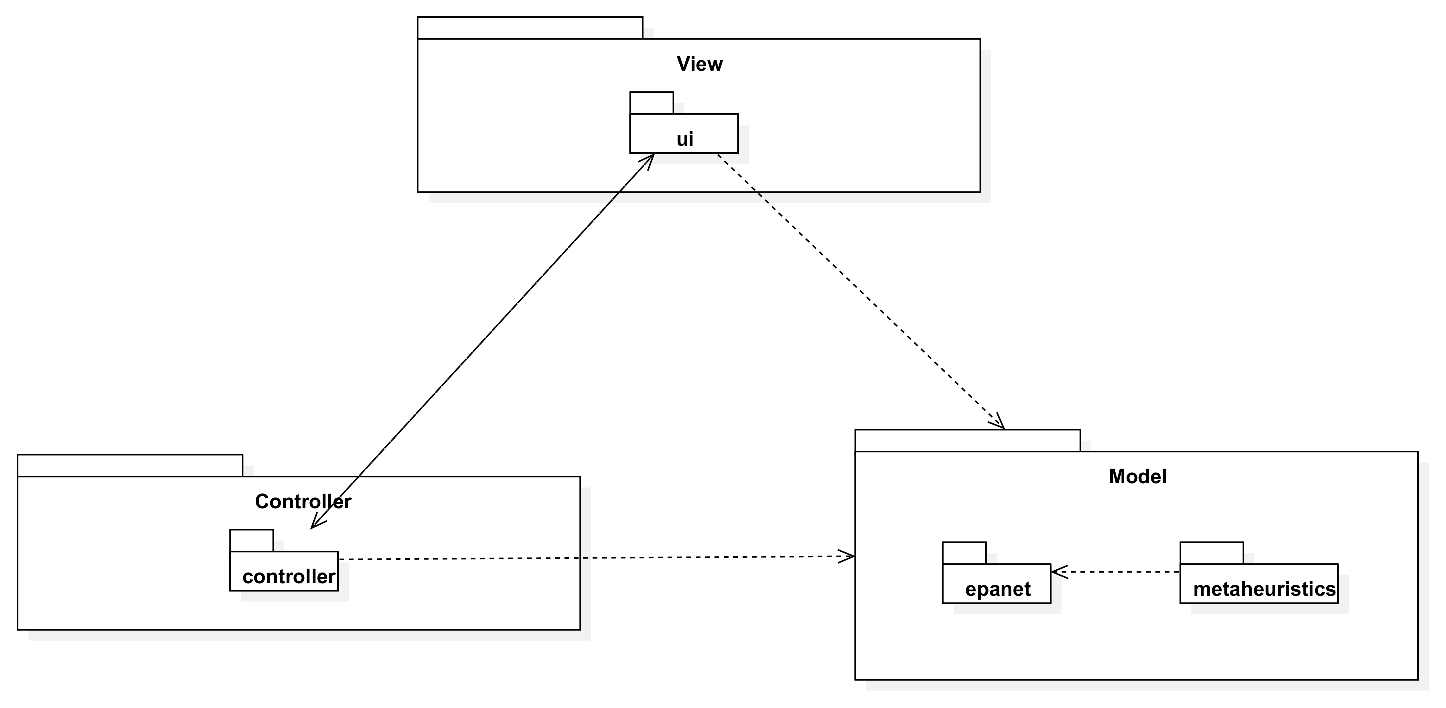
\includegraphics[width=\textwidth]{Capitulo4/assets/arquitectura_logica.eps}
	\centering
	\caption{Arquitectura l�gica Modelo-Vista-Controlador}
	\label{fig:arq_logica}
\end{figure}

A continuaci�n se presentar�n los dise�os relaci�nados por cada una de las funcionalidades escogidas con anterioridad.

\paragraph{Funcionalidad 1:} Para implementar esta funcionalidad es necesario abstraer en un conjunto de clases los datos almacenados en el archivo de configuraci�n de red. La Figura \ref{fig:dia_clase_network} muestra el diagrama de clases de las clases sobre la que almacenan los datos al momento de cargar la red. 


\begin{figure}[H]
  \centering
  \includegraphics[width=\textwidth]{Capitulo4/assets/d_clases_network.eps}
	\caption{Diagrama de clases de la abstracci�n de la red.}
	\label{fig:dia_clase_network}
\end{figure}

El diagrama de la Figura \ref{fig:dia_sec_visualizacion} muestra el conjunto de clases y los mensajes de la clases que interact�an con la clase \textit{Network} con el fin de visualizar la red. 

\begin{figure}[h]
  \centering
  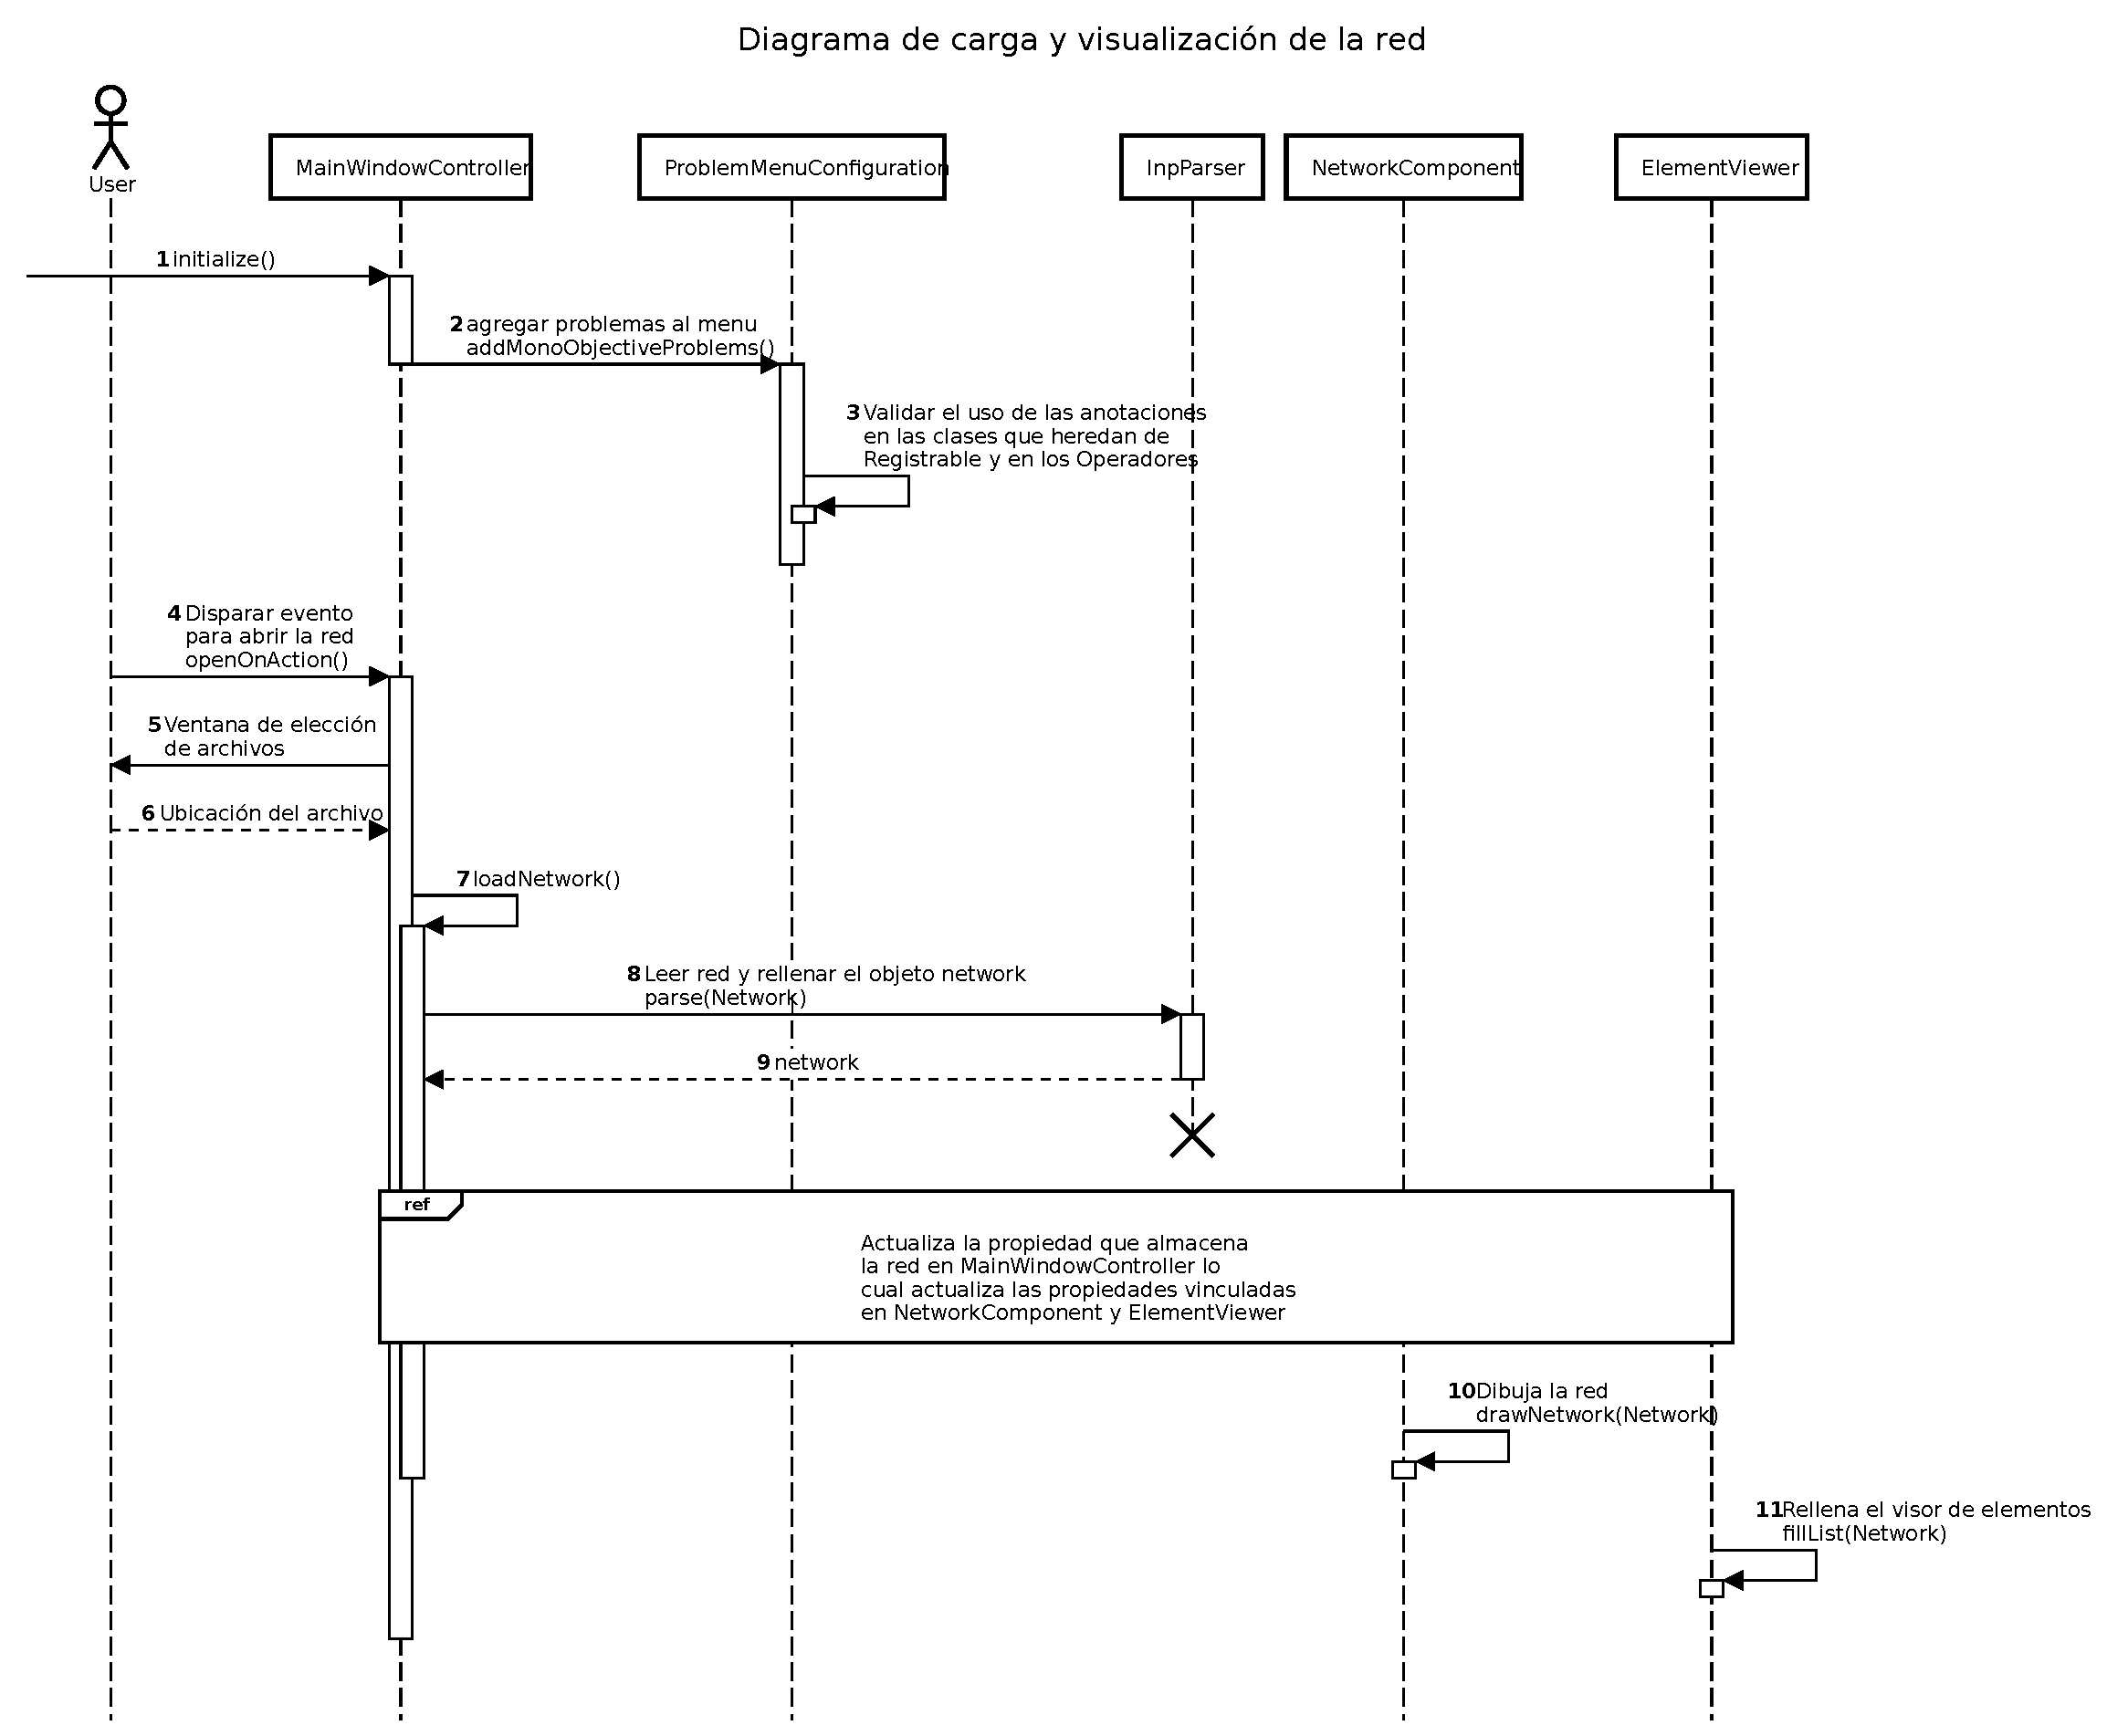
\includegraphics[width=\textwidth]{Capitulo4/assets/d_sec_visualizacion.eps}
	\caption{Diagrama de secuencia de la carga y visualizaci�n de la red.}
	\label{fig:dia_sec_visualizacion}
\end{figure}

\paragraph{Funcionalidad 2:} Esta es una de las funcionalidades ligada al modulo metaheur�stica y debido a uno de los requisitos establecidos por el cliente de que la aplicaci�n debe poder extender el n�mero de algoritmos, operadores y problemas implementados es necesario implementar una jerarqu�a de clases que facilite lo anteriormente mencionado. Es por ello, que se utilizo como base la jerarqu�a de clases utilizada por el Framework JMetal~\cite{Durillo2010} la cual fue adaptada para ser ocupada por esta aplicaci�n. La Figura \ref{fig:dia_class_met} corresponde a la jerarqu�a ya mencionada.


\begin{figure}[H]
  \centering
  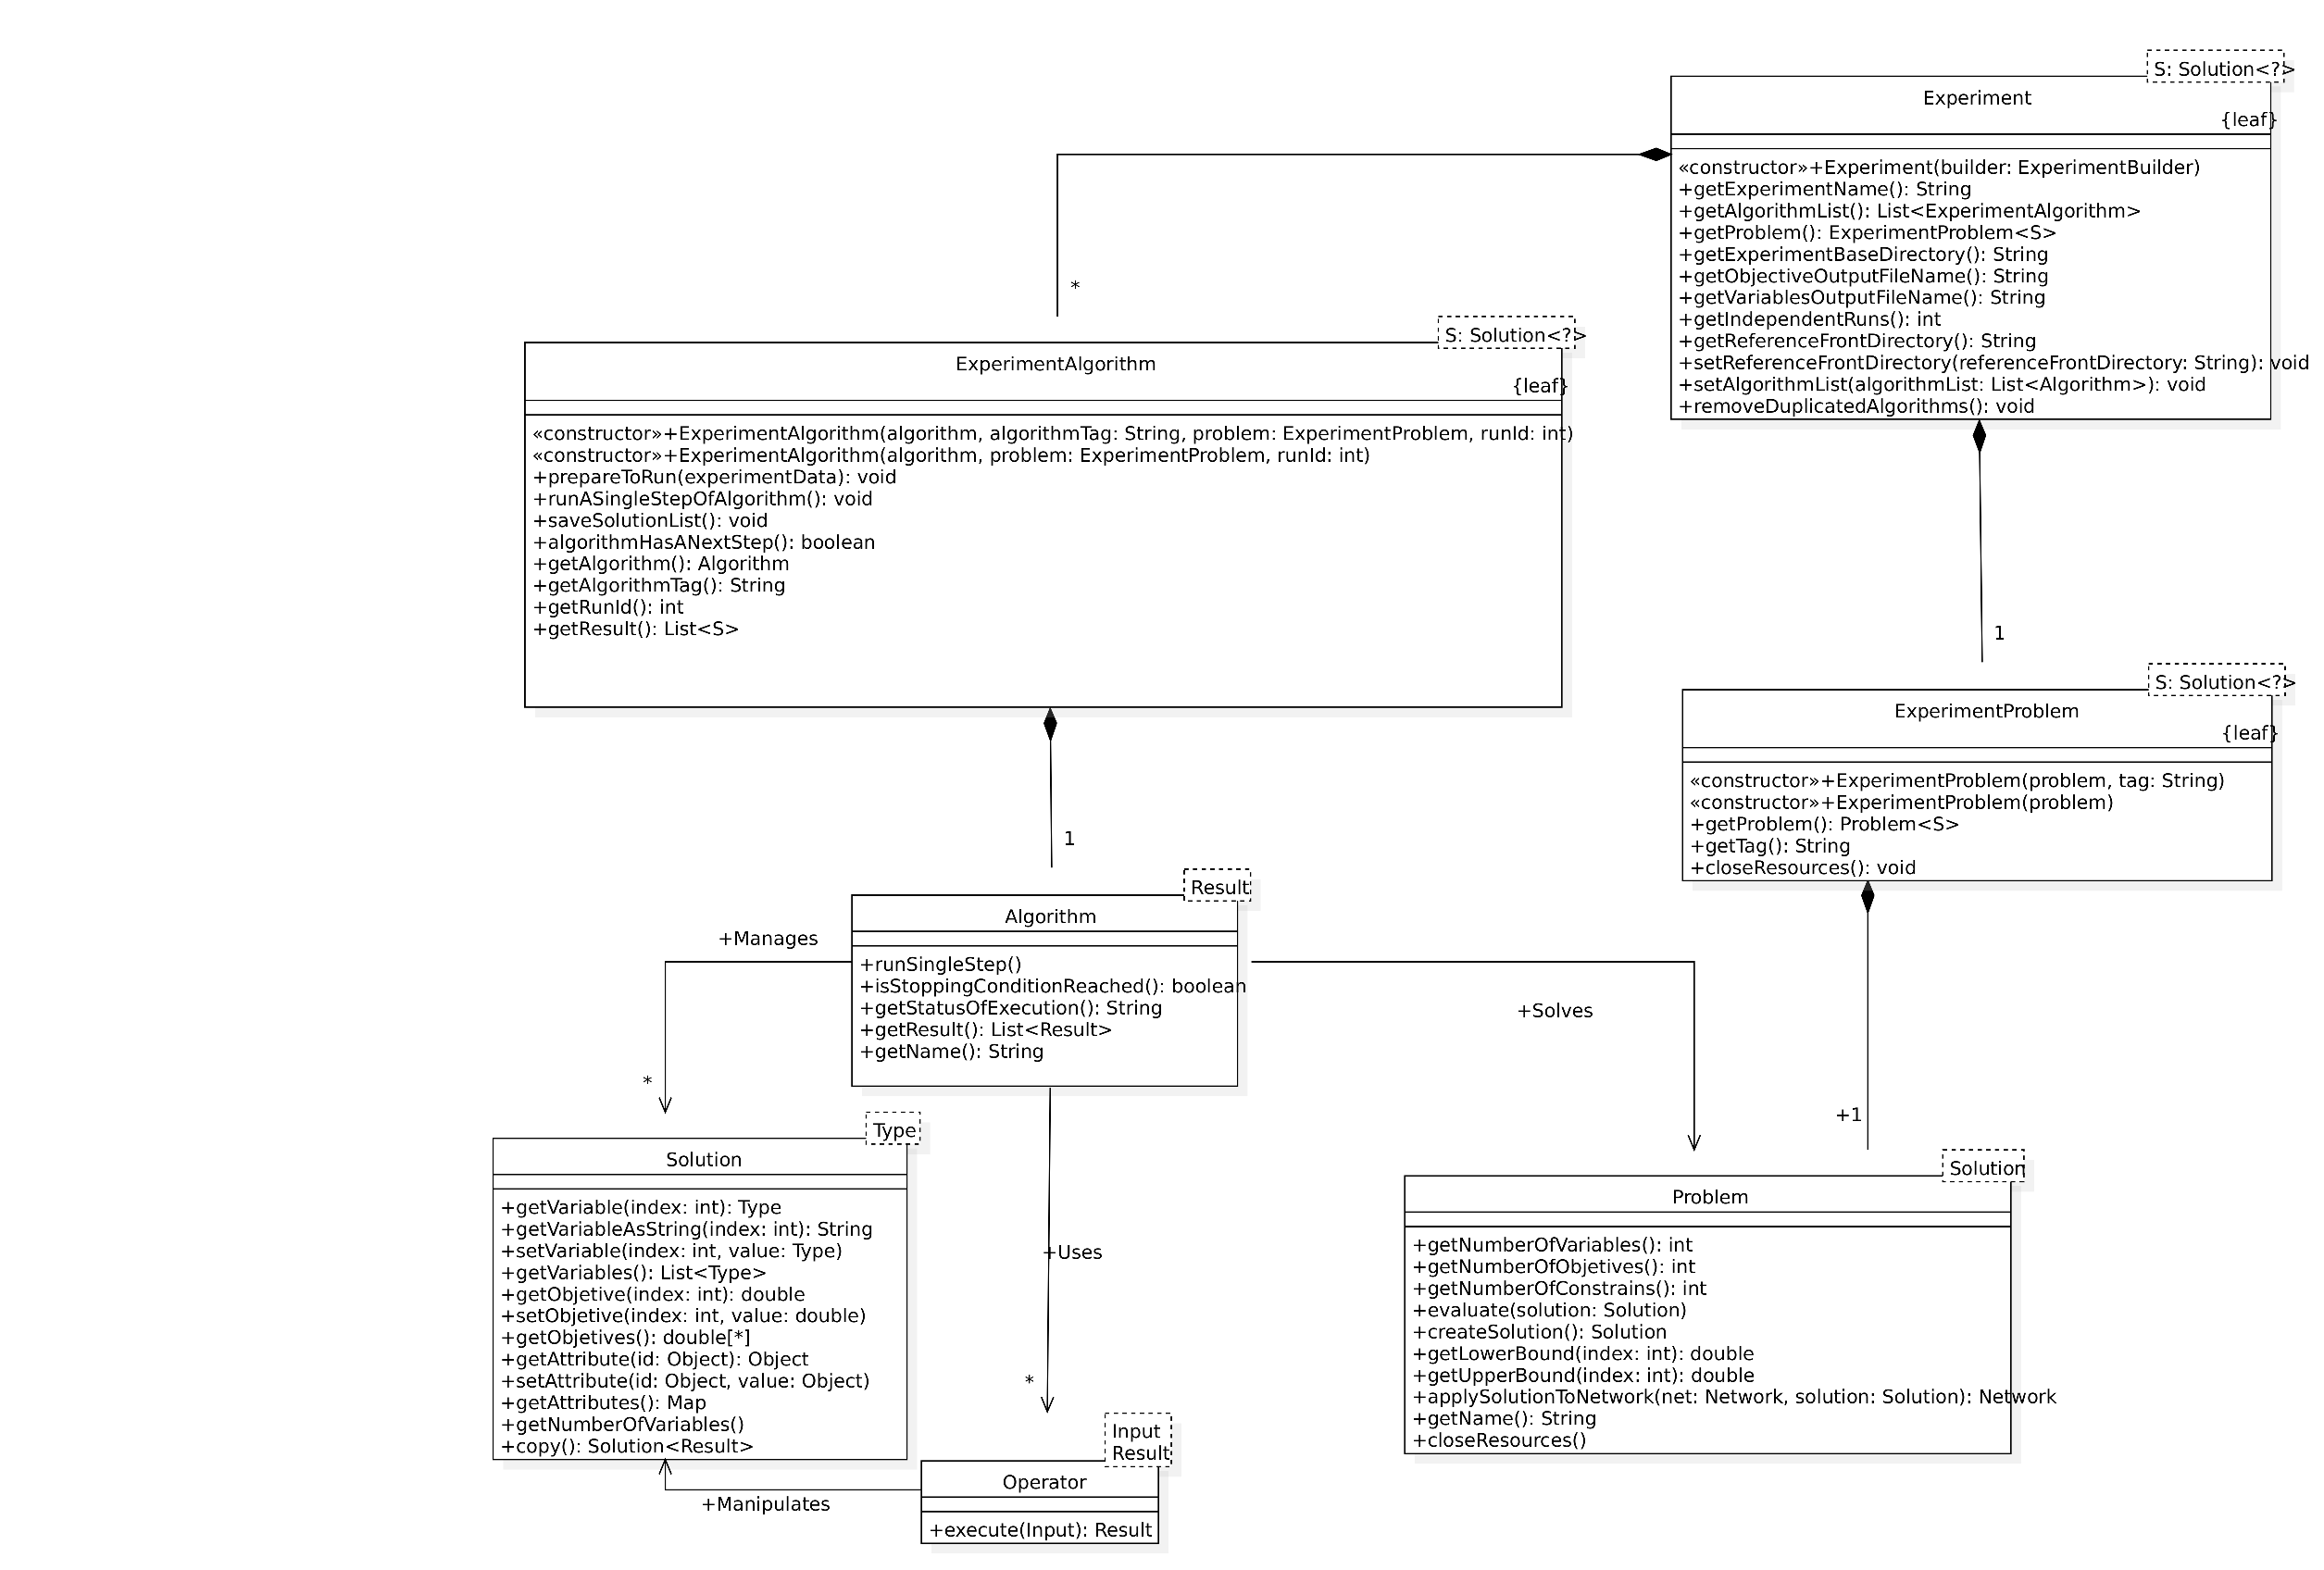
\includegraphics[width=\textwidth]{Capitulo4/assets/d_clases_metaheuristica.eps}
	\caption{Diagrama de clases modulo metaheur�stica. Modificaci�n a partir del diagrama presentado en \cite{Durillo2010}.}
	\label{fig:dia_class_met}
\end{figure}

El diagrama de secuencia de la Figura \ref{fig:dia_sec_opt} muestra la interacci�n de las clases con del modulo metaheur�sticas, con el resto de clases de la aplicaci�n.

\begin{figure}[H]
  \centering
  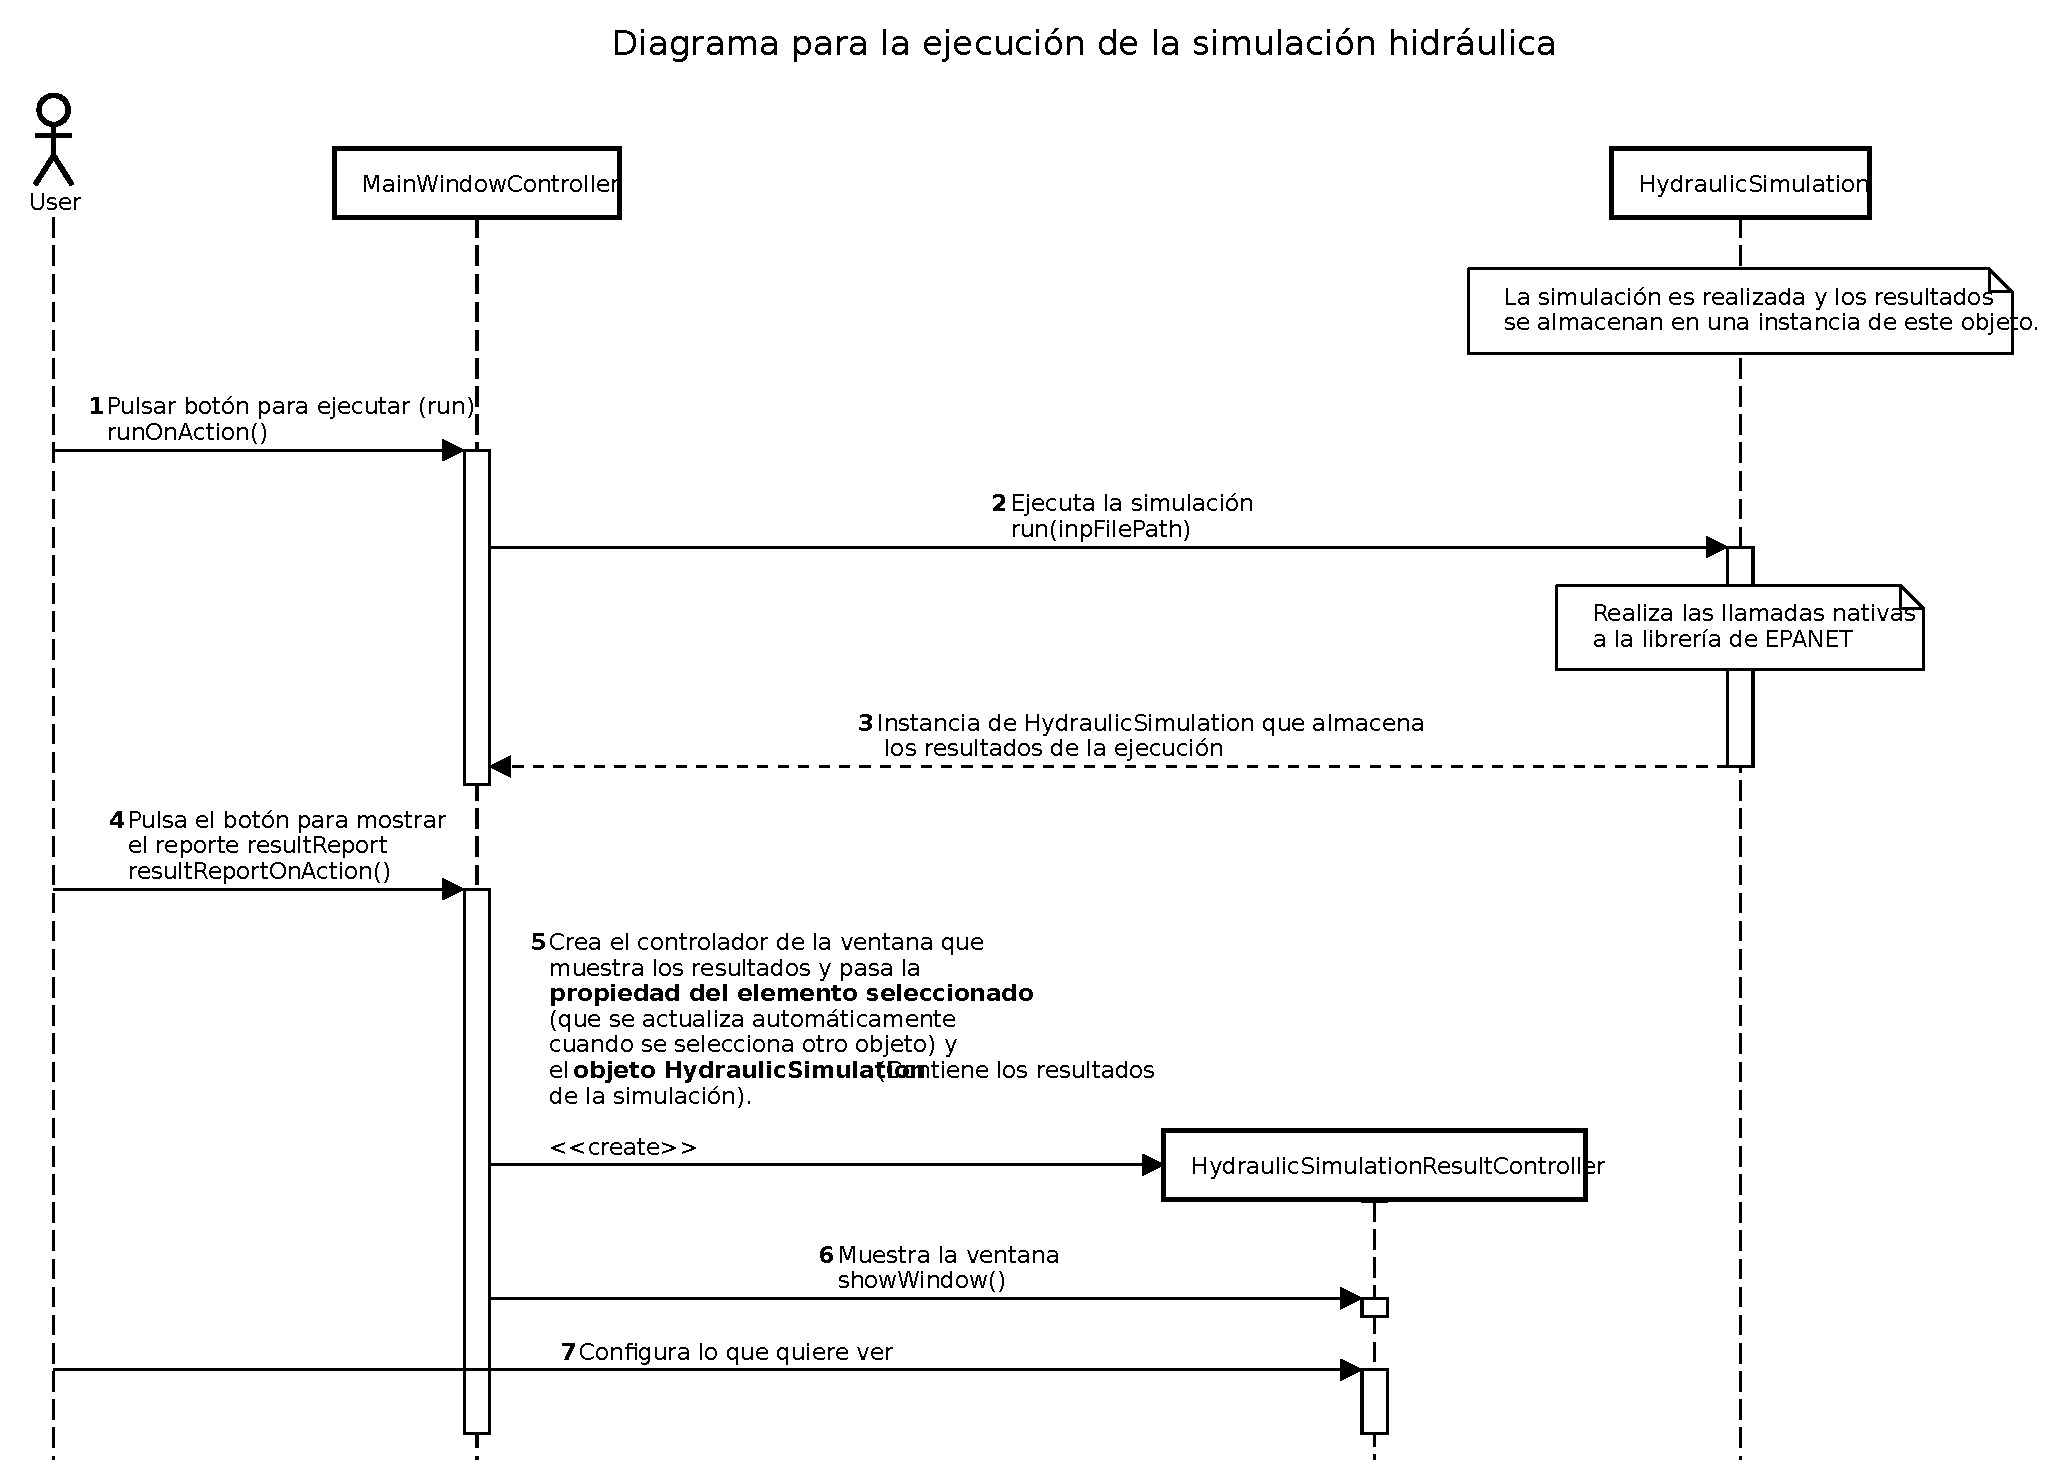
\includegraphics[width=\textwidth]{Capitulo4/assets/d_seq_simulacion-monomulti.eps}
	\caption{Diagrama de secuencia para llevar a cabo la optimizacion de los problemas.}
	\label{fig:dia_sec_opt}
\end{figure}

\paragraph{Funcionalidad 3:} Para implementar esta funcionalidad es necesario implementar un conjunto de clases las cuales guardaran los resultados de la simulaci�n para cada uno de los nodos y enlaces de una red. Estas nuevas clases son las mostradas en la Figura \ref{fig:dia_class_sim_hyd}.


\begin{figure}[H]
  \centering
  \includegraphics[width=\textwidth]{Capitulo4/assets/d_clases_hyd_simulation.eps}
	\caption{Diagrama de clases para la simulaci�n hidr�ulica}
	\label{fig:dia_class_sim_hyd}
\end{figure}

El diagrama de secuencia presentado en la Figura \ref{fig:dia_sec_sim_hyd} muestra la interacci�n entre las clases necesarias para realizar la simulaci�n hidr�ulica utilizando los valores del archivo de red cargado.

\begin{figure}[H]
  \centering
  \includegraphics[width=\textwidth]{Capitulo4/assets/d_seq_simulacion-hidraulica.eps}
	\caption{Diagrama de secuencia para realizar la simulaci�n hidr�ulica}
	\label{fig:dia_sec_sim_hyd}
\end{figure}

En el \textbf{Anexo B} se puede ver la el documento de dise�o de la aplicaci�n.

\section{Implementaci�n}
Con la fase de dise�o finalizada, se procede a realizar la fase de implementaci�n. Durante esta fase se genera el c�digo de la aplicaci�n y se genera el manual de usuario.

La aplicaci�n fue desarrollada en el lenguaje Java version 1.8. Con el fin de crear las interfaces de usuario se utilizo el Framework JavaFX.

En el cuadro~\ref{fig:actualizacion_implementacion} se presenta las tareas realizadas durante esta fase del desarrollo del software.

\begin{longtable}{||c| m{10cm}||}
  \caption{Actividades fase de implementaci�n}
  \label{fig:actualizacion_implementacion}
  \endfirsthead
  \hline
  N� Iteraci�n & Descripci�n\\ [0.5ex] 
  \hline\hline
  1 & Se codifican las clases para cargar la red \textit{Network}.\\
  \hline
  2 & Se codifican las clases del modulo metaheuristica. \newline Se implementa el algoritmo gen�tico.\newline Se implementa la codificaci�n del problema monoobjetivo \textit{Pipe Optimizing}. \newline Se implementan los operadores IntegerRandomMutation, SBXCrossover, IntegerPolinomialMutation, IntegerRangeRandomMutation y UniformSelection.\\
  \hline
  3 & Se implementan la interfaz de usuario principal. \newline Se implementa el componente para visualizar la red \newline Se implementa la interfaz de configuraci�n del problema. \newline Se implementa la interfaz de visualizaci�n de resultados de optimizaci�n. \newline Se implementa la interfaz que muestra el gr�fico con los resultados de la optimizacion. \newline Se implementa la funcionalidad para guardar las soluciones en TSV. \newline Se implementa funcionalidad para exportar la soluci�n escogida como un inp(Formato del archivo de configuraci�n de red). \\
  \hline
  4 & Se agrega el algoritmo NSGAII. \newline Se implementa la codificaci�n del problema multiobjetivo \textbf{Pumping Scheduling}.\\
  \hline
  5 & Se modifican las clases y archivos relacionados a la interfaces de usuario. \newline Se implementa la funcionalidad para realizar m�ltiples simulaciones independientes de un mismo algoritmo para los problemas multiobjetivos (Experimentos). \newline Se implementa la funcionalidad para realizar la simulaci�n usando los valores del archivo de red.\\
  \hline
  6 & Se modifica el componente de visualizaci�n de red para mostrar para cada tipo de elemento que conforma la red un s�mbolo distinto. \newline Se implementa funcionalidad para mostrar una leyenda de los s�mbolos. \newline Se implementa ventana de configuraci�n de la aplicaci�n. \newline Se implementa la funcionalidad para realizar m�ltiples simulaciones independientes para los problemas monoobjetivo (Se adapta para utilizar los Experimentos antes utilizados solo en problemas multiobjetivos).\newline Se permite agregar valores por defecto en la ventana de configuraci�n del problemas. \newline Se implementa la funcionalidad para exportar resultados a un Excel.\\
  \hline
\end{longtable}

A continuaci�n se presentara para cada una de las funcionalidades escogidas las interfaces implementadas.

\paragraph{Funcionalidad 1}: La Figura~\ref{fig:ventana_visualizacion} muestra la ventana de visualizaci�n de la red.

\begin{figure}[H]
  \centering
  \includegraphics[width=\textwidth]{Capitulo4/assets/VisualizacionRed.png}
	\caption{Ventana principal de la aplicaci�n donde se visualiza la red}
	\label{fig:ventana_visualizacion}
\end{figure}

\paragraph{Funcionalidad 2}: Las Figuras~\ref{fig:ventana_descripcion},~\ref{fig:ventana_configuracion_problema},~\ref{fig:ventana_operador},~\ref{fig:ventana_retroalimentacion} y~\ref{fig:ventana_resultados_opt} muestran las ventana utilizadas durante el cumplimiento de esta funcionalidad.

\begin{figure}[H]
  \centering
  \includegraphics[width=\textwidth]{Capitulo4/assets/ConfiguracionProblema1.png}
	\caption{Ventana de descripci�n del problema.}
	\label{fig:ventana_descripcion}
\end{figure}

\begin{figure}[H]
  \centering
  \includegraphics[width=\textwidth]{Capitulo4/assets/ConfiguracionProblema2.png}
	\caption{Ventana de configuraci�n del problema.}
	\label{fig:ventana_configuracion_problema}
\end{figure}

\begin{figure}[H]
  \centering
  \includegraphics[width=\textwidth]{Capitulo4/assets/ConfiguracionProblema3.png}
	\caption{Ventana de configuraci�n de par�metros del operador \textit{UniformSelection}}
	\label{fig:ventana_operador}
\end{figure}

\begin{figure}[H]
  \centering
  \includegraphics[width=\textwidth]{Capitulo4/assets/VentanaDeEjecucionMono.png}
	\caption{Ventana del retroalimentaci�n mostrada durante la ejecuci�n}
	\label{fig:ventana_retroalimentacion}
\end{figure}

\begin{figure}[H]
  \centering
  \includegraphics[width=\textwidth]{Capitulo4/assets/VentanaDeResultadosMono.png}
	\caption{Ventana de resultados generada cuando termina la ejecuci�n para el problema monoobjetivo Pipe Optimizing}
	\label{fig:ventana_resultados_opt}
\end{figure}

\paragraph{Funcionalidad 3}: La Figura~\ref{fig:ventana_simulacion_hyd} muestra la ventana con los resultados de una simulaci�n hidr�ulica para la red cargada.


\begin{figure}[H]
  \centering
  \includegraphics[width=\textwidth]{Capitulo4/assets/VentanaDeSimulacionHidraulica.png}
	\caption{Ventana de simulaci�n hidr�ulica utilizando los valores del archivo de red}
	\label{fig:ventana_simulacion_hyd}
\end{figure}
\section{Pruebas}

En esta ultima fase del proceso de desarrollo se procede a evaluar las funcionalidades implementadas.

Para la evaluaci�n de las funcionalidades de la aplicaci�n se aplican una serie de casos de prueba. Estos casos de prueba se dividen en dos categor�a. Los casos de prueba utilizados para pruebas automatizadas y aquellos casos de prueba utilizados para pruebas manuales. 

Los casos de prueba automatizados son aquellos realizados utilizando herramientas que permiten automatizar las tareas necesarias para evaluar los elementos que componen el software. Estas pruebas se llevan a cabo sobre los elementos del software como las clases o funciones implementadas. Estos casos de prueba se identificaron usando diversos m�todos de testeo como herramienta para especificar los casos que deben ser evaluados. Los m�todos utilizados principalmente para identificar los casos de prueba fueron los de caja negra y los de caja blanca.

Los caso de prueba manuales se refieren a aquellas pruebas realizadas con la ayuda humana. Es decir, realizados personalmente por un ser humano. Estos casos de prueba son utilizados principalmente para comprobar la funcionalidades de la interfaz gr�fica donde automatizar las pruebas tiene una mayor complejidad.

% \begin{table}
%    \begin{center}
%        \caption{Actividades fase de pruebas}
%        \bigskip
%        \begin{tabular}{||c|c||}
%             \hline
%             N� Iteraci�n & Tareas\\ [0.5ex] 
%             \hline\hline
%             1 & \\
%             2 & \\
%             3 & \\
%             4 & \\
%             5 & \\
%             6 & \\
%             \hline
%        \end{tabular}
%        \label{fig:cambios_pruebas}
%    \end{center}
% \end{table}

A continuaci�n se presentan las pruebas realizadas que abarcan a cada una de las funcionalidades escogidas.

\paragraph{Funcionalidad 1}: El Cuadro~\ref{fig:MT001} muestra la especificaci�n formal para el caso de prueba manual realizado sobre esta funcionalidad.
\paragraph{Funcionalidad 2}: Los Cuadros~\ref{fig:MT002} y \ref{fig:MT003} muestran la especificaci�n para los casos de prueba manuales de esta funcionalidad.
\paragraph{Funcionalidad 3}: Los Cuadros~\ref{fig:MT013}, \ref{fig:MT014}, \ref{fig:MT015} y \ref{fig:MT016} muestran la especificaci�n para los casos de prueba manuales de esta funcionalidad.

\begin{prueba}[fig:MT001][Especificaci�n caso de prueba manual MT001][0.8\textwidth]
    \TestID{MT001}
    \Titulo{Visualizaci�n de la red.}
    \Caracteristica{Mostrar visualizaci�n de la red.}
    \Objetivo{Confirmar que la red puede ser leida desde un archivo ``.inp'' y ser visualizada en la applicaci�n.}
    \Configuracion{El equipo tiene la applicaci�n JHawanetFramework lista para ejecutar.}
    \DatosPrueba{%
        inp: hanoi-Frankenstein.inp
    }
    \AccionesPrueba{%
        1. Abrir JHawanetFramework\\
        2. Cargar archivo de red.
    }
    \ResultadosEsperados{El sistema muestra la red leida desde un archivo inp gr�ficamente en la applicaci�n.}
\end{prueba}

\begin{prueba}[fig:MT002][Especificaci�n caso de prueba manual MT002][0.8\textwidth]
    \TestID{MT002}
    \Titulo{Optimizaci�n monoobjetivo realizada completamente.}
    \Caracteristica{Realizar simulaci�n monoobjetivo.}
    \Objetivo{Confirmar que se puede llevar a cabo la resoluci�n del problema \textit{PipeOptimizing} sobre la red abierta.}
    \Configuracion{El equipo tiene la applicaci�n JHawanetFramework lista para ejecutar.}
    \DatosPrueba{%
        independentRun = 10\\
        Archivo inp: hanoi-Frankenstein.inp\\
        Archivo gama: hanoiHW.Gama
    }
    \AccionesPrueba{%
        1. Abrir JHawanetFramework\\
        2. Cargar archivo de red.\\
        3. Seleccionar el problema \textit{PipeOptimizing del men�}.\\
        4. Configurar el problema usando la ventana de configuraci�n.\\
        5. Realizar la optimizaci�n.
    }
    \ResultadosEsperados{Al terminar la optimizaci�n el sistema muestra una interfaz con las soluciones generadas por la optimizaci�n. Debe haber tantas soluciones como el numero de configuraciones independientes (\textit{independentRun}).}
\end{prueba}

\begin{prueba}[fig:MT003][Especificaci�n caso de prueba manual MT003][0.8\textwidth]
    \TestID{MT003}
    \Titulo{Optimizaci�n monoobjetivo cancelada.}
    \Caracteristica{Realizar simulaci�n monoobjetivo.}
    \Objetivo{Confirmar que se puede llevar a cabo la resoluci�n del problema \textit{PipeOptimizing} sobre la red abierta y que se puede cancelar el proceso  cerrando la ventana o pulsando cancelar.}
    \Configuracion{El equipo tiene la applicaci�n JHawanetFramework lista para ejecutar.}
    \DatosPrueba{%
        Archivo inp: hanoi-Frankenstein.inp\\
        Archivo gama: hanoiHW.Gama
    }
    \AccionesPrueba{%
        1. Abrir JHawanetFramework\\
        2. Cargar archivo de red.\\
        3. Seleccionar el problema \textit{PipeOptimizing del men�}.\\
        4. Configurar el problema usando la ventana de configuraci�n.\\
        5. Realizar la optimizaci�n.
    }
    \ResultadosEsperados{Al cancelar la busqueda de soluciones la ventana de estado indica que la optimizaci�n a sido detenida.}
\end{prueba}

\begin{prueba}[fig:MT013][Especificaci�n caso de prueba manual MT013][0.8\textwidth]
    \TestID{MT013}
    \Titulo{Simulaci�n hidr�ulica sobre red de un solo tiempo.}
    \Caracteristica{Realizar simulaci�n con configuraci�n de archivo de red.}
    \Objetivo{Confirmar que se puede realizar la simulaci�n utilizando los valores del archivo de red.}
    \Configuracion{El equipo tiene la applicaci�n JHawanetFramework lista para ejecutar.}
    \DatosPrueba{%
        Archivo inp: hanoi-Frankenstein.inp\\
        Archivo gama: hanoiHW.Gama
    }
    \AccionesPrueba{%
        1. Abrir JHawanetFramework\\
        2. Cargar archivo de red.\\
        3. Pulsar bot�n \textit{Execute} de la ventana principal.
    }
    \ResultadosEsperados{
        Ejecuci�n realizada sin ningun error.
    }
\end{prueba}

\begin{prueba}[fig:MT014][Especificaci�n caso de prueba manual MT014][0.8\textwidth]
    \TestID{MT014}
    \Titulo{Ver resultados de la simulaci�n hidr�ulica de un solo tiempo}
    \Caracteristica{Realizar simulaci�n con configuraci�n de archivo de red.}
    \Objetivo{Confirmar que se puede visualizar los resultados de la simulaci�n realizada.}
    \Configuracion{El equipo tiene la applicaci�n JHawanetFramework lista para ejecutar.}
    \DatosPrueba{%
        Archivo inp: hanoi-Frankenstein.inp\\
        Archivo gama: hanoiHW.Gama
    }
    \AccionesPrueba{%
        1. Abrir JHawanetFramework\\
        2. Cargar archivo de red.\\
        3. Pulsar bot�n \textit{Execute} de la ventana principal.\\
        4. Pulsar bot�n \textit{Results} de la ventana principal.
    }
    \ResultadosEsperados{
        Una interfaz que permite seleccionar si se quieren ver los resultados para los enlaces o los nodos.
    }
\end{prueba}

\begin{prueba}[fig:MT015][Especificaci�n caso de prueba manual MT015][0.8\textwidth]
    \TestID{MT015}
    \Titulo{Simulaci�n hidr�ulica sobre red de mas de un tiempo.}
    \Caracteristica{Realizar simulaci�n con configuraci�n de archivo de red.}
    \Objetivo{Confirmar que se puede realizar la simulaci�n utilizando los valores del archivo de red.}
    \Configuracion{El equipo tiene la applicaci�n JHawanetFramework lista para ejecutar.}
    \DatosPrueba{%
        Archivo inp: Vanzyl.inp\\
        Archivo gama: VanzylConfiguration.json
    }
    \AccionesPrueba{%
        1. Abrir JHawanetFramework\\
        2. Cargar archivo de red.\\
        3. Pulsar boton \textit{Execute} de la ventana principal.
    }
    \ResultadosEsperados{
        Ejecuci�n realizada sin ningun error.
    }
\end{prueba}

\begin{prueba}[fig:MT016][Especificaci�n caso de prueba manual MT016][0.8\textwidth]
    \TestID{MT016}
    \Titulo{Ver resultados de la simulaci�n hidr�ulica de mas de un tiempo}
    \Caracteristica{Realizar simulaci�n con configuraci�n de archivo de red.}
    \Objetivo{Confirmar que se puede visualizar los resultados de la simulaci�n realizada.}
    \Configuracion{El equipo tiene la applicaci�n JHawanetFramework lista para ejecutar.}
     \DatosPrueba{%
        Archivo inp: Vanzyl.inp\\
        Archivo gama: VanzylConfiguration.json
    }
    \AccionesPrueba{%
        1. Abrir JHawanetFramework\\
        2. Cargar archivo de red.\\
        3. Pulsar bot�n \textit{Execute} de la ventana principal.\\
        4. Pulsar bot�n \textit{Results} de la ventana principal.
    }
    \ResultadosEsperados{
        Una interfaz que permite seleccionar si se quieren ver los resultados para los enlaces o los nodos. Adicionalmente, permite escoger el tiempo de simulaci�n y listar los resultados para todos los tiempos de un elemento de la red espec�fico.
    }
\end{prueba}

La especificaci�n de las restantes pruebas realizadas se encuentra en el \textbf{Anexo~\ref{appendix:prueba}}.
\chapter{Evaluaci�n de la soluci�n}

En este cap�tulo se da a conocer la metodolog�a de evaluaci�n y su aplicaci�n, detallando las fases y los resultados de �stas, con el fin de evaluar la soluci�n implementada.


\section{Metodolog�a de evaluaci�n}

La metodolog�a que se ha escogido para realizar este an�lisis consiste en el estudio de caso. Para llevar a cabo este estudio de caso se comienza realizando el dise�o del caso de estudio, luego se realiza la recolecci�n de datos, el an�lisis de los datos recolectados y finalmente de reportan los resultados junto con las conclusiones del estudio.

En el dise�o del caso, se define el caso a estudiar, los objetivos, el protocolo para conducir el estudio, las caracter�sticas que se quieren evaluar y los sujetos de prueba o unidad de an�lisis.

En la recolecci�n de datos, se aplica el instrumento a la unidad de an�lisis.

Durante la etapa de an�lisis, se procesan los datos presentando una serie de gr�ficas que ayudar�n a visualizar de mejor manera la informaci�n recolectada.

Finalmente, durante la etapa de reporte se presentar�n las conclusiones de la aplicaci�n del caso de estudio.

\section{Dise�o del caso de estudio}

En esta secci�n, como se menciono anteriormente, se detalla el plan de acci�n previo a la aplicaci�n del caso.

\subsection{Elecci�n del caso}

El caso a evaluar consiste en el software desarrollado durante este proyecto de titulaci�n. Como ya se sabe, es un software que permite buscar soluciones a problemas hidr�ulicos utilizando algoritmos metaheur�sticos.

\subsection{Objetivos de la investigaci�n}

El estudio que se quiere llevar a cabo es un estudio del tipo cualitativo, transversal y descriptivo, con el cual se busca comprender como el sistema desarrollado se desempe�a en la practica y su grado de aceptaci�n.

Como pregunta de investigaci�n se establece la siguiente:

\begin{center}
    \textit{�C�mo el sistema desarrollado trabaja en la pr�ctica?}
\end{center}

\subsection{Caracter�sticas a evaluar}
\label{cap:caracteristicas_a_evaluar}

Las caracter�sticas que se buscan evaluar mediante la aplicaci�n del caso de estudio son las siguientes:

\begin{itemize}
    \item \textbf{Funcionalidad}: Con esta caracter�stica se busca evaluar lo que la aplicaci�n puede hacer, es decir, si el sistema cumple con las operaciones que se busca realizar con el programa.
    \item \textbf{Facilidad de uso}: Esta caracter�stica busca medir la usabilidad del software, es decir, que tan f�cil es de usar y comprender la aplicaci�n. 
    \item \textbf{Utilidad}: Con este criterio se busca medir el valor de la aplicaci�n. Con valor, nos referimos a si las funcionalidades implementadas por el sistema son de utilidad para quien haga uso de soluci�n.
\end{itemize}

 La medici�n de cada una de estas caracter�sticas se lleva a cabo usando encuestas.

\subsection{Protocolo para conducir el estudio de caso}
El objetivo de este protocolo es establecer una gu�a para realizar la recolecci�n de datos.

Debido a la complejidad de coordinar y agendar una reuni�n se opt� por realizar la recolecci�n de datos de manera as�ncrona.

El protocolo para llevar a cabo la evaluaci�n del sistema consiste en:

\begin{enumerate}
    \item Enviar la aplicaci�n junto con su manual a los participantes del estudio.
    \item Dar un tiempo para que el participante del estudio se interiorice con la aplicaci�n.
    \item Enviar la encuesta a los participantes.
\end{enumerate}

El instrumento utilizado para evaluar la soluci�n se encuentra en el \textbf{Anexo~\ref{appendix:evaluacion}}.

\subsection{Unidad de an�lisis}
La recopilaci�n de datos se lleva a cabo sobre profesionales con conocimientos tanto en el �rea computacional, hidr�ulica y metaheur�sticas. 

\section{Consideraciones preliminar}

\textbf{Consideraciones t�cnicas}:
En esta secci�n se mencionan algunas consideraciones preliminares t�cnicas como de usuario.
\begin{itemize}
    \item Para utilizar el software se requiere el sistema operativo Window con la versi�n de Java 1.8.
    \item Para crear una nueva red se debe usar un programa externo. Este programa es Epanet y la red debe ser exportada a un archivo .inp. Debido a que la versi�n en espa�ol y la en ingl�s de Epanet crean el archivo .inp cambiando algunas palabras claves que forman parte del archivo de configuraci�n de red exportado, se opt� por utilizar el formato de la versi�n en ingl�s de Epanet dentro del programa desarrollado.
    \item Para visualizar los resultados de la exportaci�n a un documento de Excel, se requiere dicho programa o alguna alternativa que permita visualizar las hojas de c�lculo con extensi�n .xslx.
\end{itemize}

\textbf{Consideraciones para los usuarios}:
\begin{itemize}
    \item Para poder implementar nuevos problemas y algoritmos se requiere tener conocimientos en hidr�ulica y programaci�n, as� como tambi�n en metaheur�sticas. Si no se requiere implementar nuevos elementos, los conocimientos en programaci�n no son tan necesarios, mientras que los de metaheur�sticas e hidr�ulica s�, con el objetivo de saber como interpretar los resultados.
\end{itemize}

\section{Recolecci�n de datos}
En esta secci�n se presentan los participantes del estudio y se detallan las caracter�sticas del instrumento utilizado para la obtenci�n de datos.

\subsubsection{Participantes}
Los participantes del proceso de recolecci�n de datos fueron los siguientes:

\bigskip
\textbf{Evaluador}
\begin{itemize}
    \item Gabriel Sanhueza
\end{itemize}

\textbf{Usuario}

\begin{itemize}
    \item Yamisleydi Salgueiro
    \item Marco Alsina
    \item Sergio Silva
\end{itemize}

\subsubsection{Instrumentos para la recolecci�n de los datos}

Para el proceso de recolecci�n de los datos se utilizaran encuestas. La encuesta esta dise�ada para evaluar las caracter�sticas mencionadas en la subsecci�n~\ref{cap:caracteristicas_a_evaluar}. La funcionalidad y la utilidad se eval�an usando la escala de Likert. En cuanto a la usabilidad, este se eval�a usando la escala de usabilidad de SUS.

La escala de usabilidad de SUS cuenta con 10 preguntas, las cuales a efecto de la presente evaluaci�n son:

\begin{enumerate}
    \item Creo que usar�a esta aplicaci�n frecuentemente.
    \item Encuentro esta aplicaci�n innecesariamente complejo.
    \item Creo que la aplicaci�n fue f�cil de usar.
    \item Creo que necesitar�a ayuda de una persona con conocimientos t�cnicos para usar esta aplicaci�n.
    \item Las funciones de esta aplicaci�n est�n bien integradas.
    \item Creo que la aplicaci�n es muy inconsistente.
    \item Imagino que la mayor�a de la gente aprender�a a usar esta aplicaci�n en forma muy r�pida.
    \item Encuentro que la aplicaci�n es muy dif�cil de usar.
    \item Me siento confiado al usar esta aplicaci�n.
    \item Necesit� aprender muchas cosas antes de ser capaz de usar esta aplicaci�n.
\end{enumerate}

La encuesta aplicada se encuentra en el \textbf{Anexo~\ref{appendix:evaluacion}}.

\section{An�lisis de datos}
En esta secci�n se presenta el an�lisis de los datos. El an�lisis se realiza de manera independiente por cada una de las caracter�sticas a evaluar, en donde se muestran los resultados utilizando herramientas como gr�ficos y tablas. Adicionalmente, se provee una interpretaci�n de los resultados.

\subsection{Resultado de la evaluaci�n de la soluci�n}


\section{Conclusiones del estudio}



%% ambiente glosario
\begin{glosario}
  \item[RDA] Red de distribuci�n de agua potable
  \item[GA] Algoritmo Gen�tico
  \item[NSGAII] Non-Dominated Sorting Genetic Algorithm II
\end{glosario}


%% genera las referencias
\bibliography{refs}


%% comienzo de la parte de anexos
\appendixpart

%% contenido del primer anexo
\appendix{Documento de especificaci�n de requisitos}
\label{appendix:requisito}
% \includepdf[pages=-]{Anexos/docreq.pdf}

%% contenido del segundo anexo
\appendix{Documento de dise�o}
\label{appendix:diseno}

% \includepdf[pages=-]{Anexos/docdisen.pdf}

\appendix{Manual de usuario}
\label{appendix:manual}

% \includepdf[pages=-]{Anexos/manual.pdf}

\appendix{Documento de casos de prueba}
\label{appendix:prueba}

% \includepdf[pages=-]{Anexos/doccu.pdf}

\appendix{Cuestionario para la evaluaci�n de la aplicaci�n}
\label{appendix:evaluacion}

% \includepdf[pages=-]{Anexos/form.pdf}

%% fin
\end{document}

   

